% !TEX root = report.tex

% !TEX root = ../report.tex

\documentclass[a4paper, 14pt]{extreport}

\usepackage{cmap}
\usepackage[T2A,T1]{fontenc}
\usepackage[utf8]{inputenc}
\usepackage[english,russian]{babel}
\usefont{T2A}{ftm}{m}{sl}

\usepackage{setspace}
\onehalfspacing % Полуторный интервал

\frenchspacing
\usepackage{indentfirst}
\setlength\parindent{1.25cm}

\usepackage{microtype} % настройка переносов и предотвращение выхода текста за поля
\emergencystretch=1em
\usepackage{shellesc}
\usepackage{amssymb,amsfonts,amsmath,mathtext,cite,enumerate,float}
\usepackage{pgfplots}
\usepackage{graphicx}
\usepackage{svg}
\usepackage[off]{svg-extract}
\svgsetup{clean=true}
\usepackage{tocloft}
\usepackage{listings}
\usepackage{caption}
\usepackage{tempora}
\usepackage{titlesec}
\usepackage{geometry}
\usepackage{indentfirst}
\usepackage{pdfpages}
\usepackage{enumerate,letltxmacro}
\usepackage{threeparttable}
\usepackage[hidelinks,bookmarks=false]{hyperref}
\usepackage{url}
\def\UrlBreaks{\do\/\do-\do_\do.\do:\do=\do?\do\&\do\#\do\%}
\usepackage{flafter}
\usepackage{enumitem}
\usepackage{multirow}
\usepackage{longtable}
\usepackage[toc]{appendix}
\usepackage{wrapfig}
\usepackage{zref-totpages}
\usepackage{makecell}

\usepackage[figure,table]{totalcount}
\usepackage{lastpage}

\setlist{nosep}

\newcommand{\rpzheading}[1]{\begin{center}
		\LARGE\bfseries{#1}
	\end{center}}
\newcommand{\ssr}[1]{\rpzheading{#1} \addcontentsline{toc}{chapter}{#1}  }
\newcommand{\rpzcontents}{%
	\rpzheading{СОДЕРЖАНИЕ}
	\begingroup
	\setlength{\cftbeforetoctitleskip}{0pt}
	\setlength{\cftaftertoctitleskip}{0pt}
	\def\contentsname{}
	\renewcommand{\cfttoctitlefont}{}
	\renewcommand{\cftaftertoctitle}{}
	\tableofcontents
	\endgroup}
\newcommand{\rpzcompacttable}{%
	\footnotesize
	\setlength{\tabcolsep}{3pt}
	\renewcommand{\arraystretch}{0.82}}
\newcommand{\rpzhideimportedpagenumber}{%
	\thispagestyle{empty}%
	\begin{tikzpicture}[remember picture,overlay]
		\fill[white] (current page.south west) rectangle ([yshift=1.6cm]current page.south east);
	\end{tikzpicture}}

\makeatletter
\renewcommand\LARGE{\@setfontsize\LARGE{22pt}{20}}
\renewcommand\Large{\@setfontsize\Large{20pt}{20}}
\renewcommand\large{\@setfontsize\large{16pt}{20}}
\makeatother
\RequirePackage{titlesec}
\titleformat{\chapter}[block]{\hspace{\parindent}\large\bfseries}{\thechapter}{0.5em}{\large\bfseries\raggedright}
\titleformat{name=\chapter,numberless}[block]{\hspace{\parindent}}{}{0pt}{\large\bfseries\centering}
\titleformat{\section}[block]{\hspace{\parindent}\large\bfseries}{\thesection}{0.5em}{\large\bfseries\raggedright}
\titleformat{\subsection}[block]{\hspace{\parindent}\large\bfseries}{\thesubsection}{0.5em}{\large\bfseries\raggedright}
\titleformat{\subsubsection}[block]{\hspace{\parindent}\large\bfseries}{\thesubsection}{0.5em}{\large\bfseries\raggedright}
\titlespacing{\chapter}{12.5mm}{-22pt}{10pt}
\titlespacing{\section}{12.5mm}{10pt}{10pt}
\titlespacing{\subsection}{12.5mm}{10pt}{10pt}
\titlespacing{\subsubsection}{12.5mm}{10pt}{10pt}

\makeatletter
\renewcommand{\@biblabel}[1]{#1.}
\makeatother

\geometry{left=30mm}
\geometry{right=10mm}
\geometry{top=20mm}
\geometry{bottom=20mm}

\renewcommand{\theenumi}{\arabic{enumi}}
\renewcommand{\labelenumi}{\arabic{enumi}\text{)}}
\renewcommand{\theenumii}{.\arabic{enumii}}
\renewcommand{\labelenumii}{\asbuk{enumii}\text{)}}
\renewcommand{\theenumiii}{.\arabic{enumiii}}
\renewcommand{\labelenumiii}{\arabic{enumi}.\arabic{enumii}.\arabic{enumiii}.}

\renewcommand{\cftchapleader}{\cftdotfill{\cftdotsep}}

\addto\captionsrussian{\renewcommand{\figurename}{Рисунок}}
\DeclareCaptionLabelSeparator{dash}{~---~}
\captionsetup{labelsep=dash}

\DeclareCaptionFormat{fmt}{\parbox{\linewidth}{#1#2#3}}
\captionsetup{justification=raggedleft,format=fmt,position=bottom}
\captionsetup[figure]{justification=centering,format=default,labelsep=dash}

\graphicspath{{img/}}%путь к рисункам

\newcommand{\floor}[1]{\lfloor #1 \rfloor}

\lstset{ %
	language=Go,                     % выбор языка для подсветки
	basicstyle=\small\sffamily, % размер и начертание шрифта для подсветки кода
	numbers=none,               % где поставить нумерацию строк (слева\справа)
	numberstyle=\tiny,           % размер шрифта для номеров строк
	stepnumber=1,                   % размер шага между двумя номерами строк
	showspaces=false,            % показывать или нет пробелы специальными отступами
	showstringspaces=false,      % показывать или нет пробелы в строках
	showtabs=false,             % показывать или нет табуляцию в строках
	frame=single,              % рисовать рамку вокруг кода
	tabsize=2,                 % размер табуляции по умолчанию равен 2 пробелам
	captionpos=t,              % позиция заголовка вверху [t] или внизу [b]
	breaklines=true,           % автоматически переносить строки (да\нет)
	breakatwhitespace=false, % переносить строки только если есть пробел
	escapeinside={\#*}{*)},   % если нужно добавить комментарии в коде
	abovecaptionskip=-5pt
}

\pgfplotsset{width=0.85\linewidth, height=0.5\columnwidth}

\linespread{1.3}

\def\labelitemi{---}
\setlist[itemize]{leftmargin=1.25cm, itemindent=0.65cm}
\setlist[enumerate]{leftmargin=1.25cm, itemindent=0.55cm}

\newcommand{\specialcell}[2][c]{%
	\begin{tabular}[#1]{@{}c@{}}#2\end{tabular}}

\frenchspacing

\lstset{
literate=
	{а}{{\selectfont\char224}}1
{б}{{\selectfont\char225}}1
{в}{{\selectfont\char226}}1
{г}{{\selectfont\char227}}1
{д}{{\selectfont\char228}}1
{е}{{\selectfont\char229}}1
{ё}{{\"e}}1
{ж}{{\selectfont\char230}}1
{з}{{\selectfont\char231}}1
{и}{{\selectfont\char232}}1
{й}{{\selectfont\char233}}1
{к}{{\selectfont\char234}}1
{л}{{\selectfont\char235}}1
{м}{{\selectfont\char236}}1
{н}{{\selectfont\char237}}1
{о}{{\selectfont\char238}}1
{п}{{\selectfont\char239}}1
{р}{{\selectfont\char240}}1
{с}{{\selectfont\char241}}1
{т}{{\selectfont\char242}}1
{у}{{\selectfont\char243}}1
{ф}{{\selectfont\char244}}1
{х}{{\selectfont\char245}}1
{ц}{{\selectfont\char246}}1
{ч}{{\selectfont\char247}}1
{ш}{{\selectfont\char248}}1
{щ}{{\selectfont\char249}}1
{ъ}{{\selectfont\char250}}1
{ы}{{\selectfont\char251}}1
{ь}{{\selectfont\char252}}1
{э}{{\selectfont\char253}}1
{ю}{{\selectfont\char254}}1
{я}{{\selectfont\char255}}1
{А}{{\selectfont\char192}}1
{Б}{{\selectfont\char193}}1
{В}{{\selectfont\char194}}1
{Г}{{\selectfont\char195}}1
{Д}{{\selectfont\char196}}1
{Е}{{\selectfont\char197}}1
{Ё}{{\"E}}1
{Ж}{{\selectfont\char198}}1
{З}{{\selectfont\char199}}1
{И}{{\selectfont\char200}}1
{Й}{{\selectfont\char201}}1
{К}{{\selectfont\char202}}1
{Л}{{\selectfont\char203}}1
{М}{{\selectfont\char204}}1
{Н}{{\selectfont\char205}}1
{О}{{\selectfont\char206}}1
{П}{{\selectfont\char207}}1
{Р}{{\selectfont\char208}}1
{С}{{\selectfont\char209}}1
{Т}{{\selectfont\char210}}1
{У}{{\selectfont\char211}}1
{Ф}{{\selectfont\char212}}1
{Х}{{\selectfont\char213}}1
{Ц}{{\selectfont\char214}}1
{Ч}{{\selectfont\char215}}1
{Ш}{{\selectfont\char216}}1
{Щ}{{\selectfont\char217}}1
{Ъ}{{\selectfont\char218}}1
{Ы}{{\selectfont\char219}}1
{Ь}{{\selectfont\char220}}1
{Э}{{\selectfont\char221}}1
{Ю}{{\selectfont\char222}}1
{Я}{{\selectfont\char223}}1
}


\begin{document}

% \includepdf[pages={1-}]{parts/01_title.pdf}
\setcounter{page}{4}

\begingroup
\renewcommand{\vspace}[2]{}% Gobble 2 arguments after \vspace
\def\contentsname{\begin{center}СОДЕРЖАНИЕ\end{center}}
\tableofcontents
\endgroup

% % !TEX root = ../report.tex

\ssr{ВВЕДЕНИЕ}

Онлайн-маркетплейс объединяет каталог товаров разных продавцов, оформление заказов покупателями, отзывы и административное управление данными. Для такой системы требуется база данных, которая хранит связанные данные о пользователях, товарах, заказах, отзывах и изменении цен, а также поддерживает разграничение доступа между ролями.

Целью курсового проекта является разработка базы данных онлайн-маркетплейса и приложения доступа к ней.

Для достижения поставленной цели необходимо решить следующие задачи:
\begin{itemize}
    \item провести анализ предметной области онлайн-маркетплейса и существующих решений;
    \item сформулировать требования и ограничения к разрабатываемой базе данных и приложению;
    \item выделить роли пользователей и сценарии взаимодействия с системой;
    \item спроектировать сущности базы данных, связи между ними и ограничения целостности;
    \item спроектировать ролевую модель доступа к данным;
    \item спроектировать триггеры журнала изменения цен и пересчёта рейтингов;
    \item спроектировать хранимую функцию расчёта статистики продаж продавца;
    \item выбрать средства реализации базы данных и приложения доступа;
    \item реализовать базу данных, кэширование и интерфейс доступа к данным;
    \item выполнить исследование влияния индексов и Redis-кэширования на измеряемые показатели доступа к данным.
\end{itemize}

\clearpage


% !TEX root = ../report.tex

\chapter{Аналитическая часть}

В данном разделе проводится анализ предметной области онлайн-маркетплейсов, включающий:

\begin{itemize}
    \item определение понятия онлайн-маркетплейса и его отличий от классического интернет-магазина;
    \item оценку существующих решений на рынке электронной коммерции;
    \item формализацию задач, решаемых проектируемой системой;
    \item описание ролей пользователей приложения;
    \item описание структур данных, необходимых для хранения информации о товарах, заказах, пользователях и связанных сущностях.
\end{itemize}

На основе проведённого анализа формируются следующие результаты:
\begin{itemize}
    \item перечень ролей пользователей проектируемой системы;
    \item определение сценариев использования системы для каждой роли;
    \item создание диаграмм: \begin{itemize}
        \item вариантов использования;
        \item сущность-связь в нотации Чена.
    \end{itemize}
    \item выбор модели БД, достаточной для решения поставленной задачи.
\end{itemize}

% !TEX root = ../../report.tex

\section{Анализ предметной области}

\textbf{Онлайн-маркетплейс} --- электронная торговая площадка, на которой множество независимых продавцов размещают свои товары, а покупатели выбирают и заказывают их через единый интерфейс~\cite{marketplace_def}. В отличие от классического интернет-магазина, маркетплейс не владеет товарами и не осуществляет их закупку: платформа выступает посредником между продавцом и покупателем, предоставляя инфраструктуру для размещения каталога, приёма заказов и сбора обратной связи.

По данным Ассоциации компаний интернет-торговли (АКИТ), объём интернет-торговли в России по итогам 2025 года составил 11,5~трлн рублей, что соответствует росту на 28\% относительно предыдущего года~\cite{akit2025}. Доля онлайн-продаж достигла 18,8\% от всего розничного товарооборота. Маркетплейсы являются значимой частью рынка онлайн-торговли.

Ключевые бизнес-процессы маркетплейса включают:

\begin{itemize}
    \item регистрацию продавцов и размещение товаров с привязкой к категориям;
    \item просмотр каталога покупателями с возможностью фильтрации и поиска;
    \item оформление заказов с фиксацией цены на момент покупки;
    \item управление жизненным циклом заказа (от корзины до доставки);
    \item систему отзывов и рейтингов, обеспечивающую обратную связь;
    \item формирование аналитической отчётности для продавцов и аналитиков.
\end{itemize}

Рассмотренные далее маркетплейсы являются закрытыми коммерческими системами. В проектируемой системе отдельно рассматриваются каталог, заказы, отзывы, история изменения цен и отчётность продавца.


% !TEX root = ../../report.tex

\section{Анализ существующих решений}

Для определения функциональных требований к проектируемой системе проведён сравнительный анализ трёх распространённых маркетплейсов, доступных российским пользователям.

\begin{itemize}
    \item \textbf{Ozon} --- маркетплейс с интерфейсом для продавцов, покрывающим управление товарами, заказами, аналитикой и финансами. Предоставляет расширенную аналитику в личном кабинете продавца, часть функций доступна по подписке. Поддерживает раздельные рейтинги товара и продавца~\cite{ozon};
    \item \textbf{Wildberries} --- маркетплейс с личным кабинетом продавца, охватывающим товары, заказы, поставки и продвижение. Базовая аналитика встроена в платформу бесплатно; для расширенной требуются сторонние сервисы. Поддерживаются раздельные рейтинги товара и продавца~\cite{wildberries};
    \item \textbf{AliExpress} --- трансграничная торговая площадка, ориентированная на международных продавцов. Базовая аналитика доступна в кабинете продавца. Поддерживаются рейтинги товара и продавца~\cite{aliexpress}.
\end{itemize}

Критерии сравнения соответствуют характеристикам, которые используются в проектируемой системе:

\begin{enumerate}
    \item открытость модели данных;
    \item история изменения цен товара;
    \item бесплатная встроенная аналитика продаж;
    \item раздельные рейтинги товара и продавца;
    \item выделенная роль аналитика только для чтения;
    \item логистика как часть предметной области.
\end{enumerate}

Сравнение платформ по сформированным критериям приведено в таблице~\ref{tbl:comparison}.

\begin{table}[h!]
    \caption{Сравнение существующих решений}
    \label{tbl:comparison}
    \centering
    \small
    \begin{tabular}{|l|l|l|l|l|}
        \hline
        \textbf{Критерий} & \textbf{Ozon} & \textbf{Wildberries} & \textbf{AliExpress} & \makecell[l]{\textbf{Проектируемая}\\\textbf{система}} \\ \hline
        \makecell[l]{Открытость\\модели данных} & Нет & Нет & Нет & Да \\ \hline
        \makecell[l]{История\\цен товара} & \makecell[l]{Не\\раскрывается} & \makecell[l]{Не\\раскрывается} & \makecell[l]{Не\\раскрывается} & Да \\ \hline
        \makecell[l]{Бесплатная встроенная\\аналитика продаж} & Частично & Да & Да & Да \\ \hline
        \makecell[l]{Рейтинг товара\\и продавца} & Да & Да & Да & Да \\ \hline
        \makecell[l]{Выделенная роль\\аналитика\\только для чтения} & \makecell[l]{Не\\указана} & \makecell[l]{Не\\указана} & \makecell[l]{Не\\указана} & Да \\ \hline
        \makecell[l]{Логистика\\в предметной\\области} & Да & Да & Да & Нет \\ \hline
    \end{tabular}
\end{table}

Рассмотренные платформы являются закрытыми коммерческими системами.

В проектируемой системе выделяются открытая модель данных, хранение истории изменения цен и отдельная роль аналитика. Задача логистики не рассматривается.


% !TEX root = ../../report.tex

\section{Формализация задачи}

Необходимо спроектировать базу данных для онлайн-маркетплейса, обеспечивающую хранение и обработку данных о товарах, продавцах, покупателях, заказах, отзывах, категориях и адресах доставки.

Требуется разработать систему, предоставляющую пользователям интерфейсы взаимодействия с данными маркетплейса. В рамках системы должны быть предусмотрены следующие роли: гость, покупатель, продавец, администратор и аналитик.

Для указанных ролей необходимо определить сценарии взаимодействия с системой: просмотр каталога, управление товарами, оформление заказов, оставление отзывов, администрирование и формирование аналитической отчётности.

Проектируемая система ограничивается каталогом товаров, заказами, адресами доставки, отзывами и состояниями исполнения заказа. Задача логистики не рассматривается: в предметную область не включаются логистические компании, маршруты, курьеры, графики складов и события фактической передачи товара. Состояние исполнения заказа фиксируется статусами заказа.

\pagebreak


% !TEX root = ../../report.tex

\section{Описание ролей}

Исходя из анализа предметной области и требований к системе, выделены следующие роли пользователей:

\begin{enumerate}
    \item гость (неавторизованный пользователь);
    \item покупатель;
    \item продавец;
    \item администратор;
    \item аналитик.
\end{enumerate}

\textbf{Гость} --- неавторизованный пользователь, обладающий правами на просмотр каталога товаров, карточки товара (включая информацию о товаре, историю изменения цены и отзывы), а также на прохождение процедуры авторизации (регистрации или входа в систему).

\textbf{Покупатель} --- авторизованный пользователь, который, помимо возможностей гостя, может оформлять заказы (добавлять товары в корзину, выбирать адрес доставки, производить оплату) и оставлять отзывы на приобретённые товары. Каждый покупатель управляет собственными адресами доставки. Один покупатель может оставить не более одного отзыва на конкретный товар.

\textbf{Продавец} --- авторизованный пользователь, зарегистрировавший профиль компании. Продавец управляет собственными товарами (добавление, редактирование, удаление), просматривает входящие заказы и фиксирует их переходы по статусам отгрузки и доставки. Также продавцу доступна статистика продаж за указанный период.

\textbf{Администратор} --- пользователь с функциями модератора платформы. Наследует возможности гостя (просмотр каталога, карточки товара, авторизация). Администратор управляет категориями товаров (создание, редактирование, удаление), может удалять пользователей, продавцов, товары и отзывы. Также ему доступен просмотр всех заказов в системе, отчётов и статистики продаж. Администратор не создаёт товары, не оформляет заказы и не оставляет отзывы.

\textbf{Аналитик} --- пользователь, обладающий правами на чтение всех данных системы без возможности их модификации. Роль предназначена для формирования отчётов: топ товаров по продажам, динамика заказов по времени, распределение продаж по категориям.

Отдельная роль для управления складскими остатками не выделяется. Количество товара относится к данным товара, которыми управляет продавец, а резерв изменяется при обработке заказов.

Диаграмма вариантов использования приведена на рисунке~\ref{fig:usecase}.

\begin{figure}[H]
    \centering
    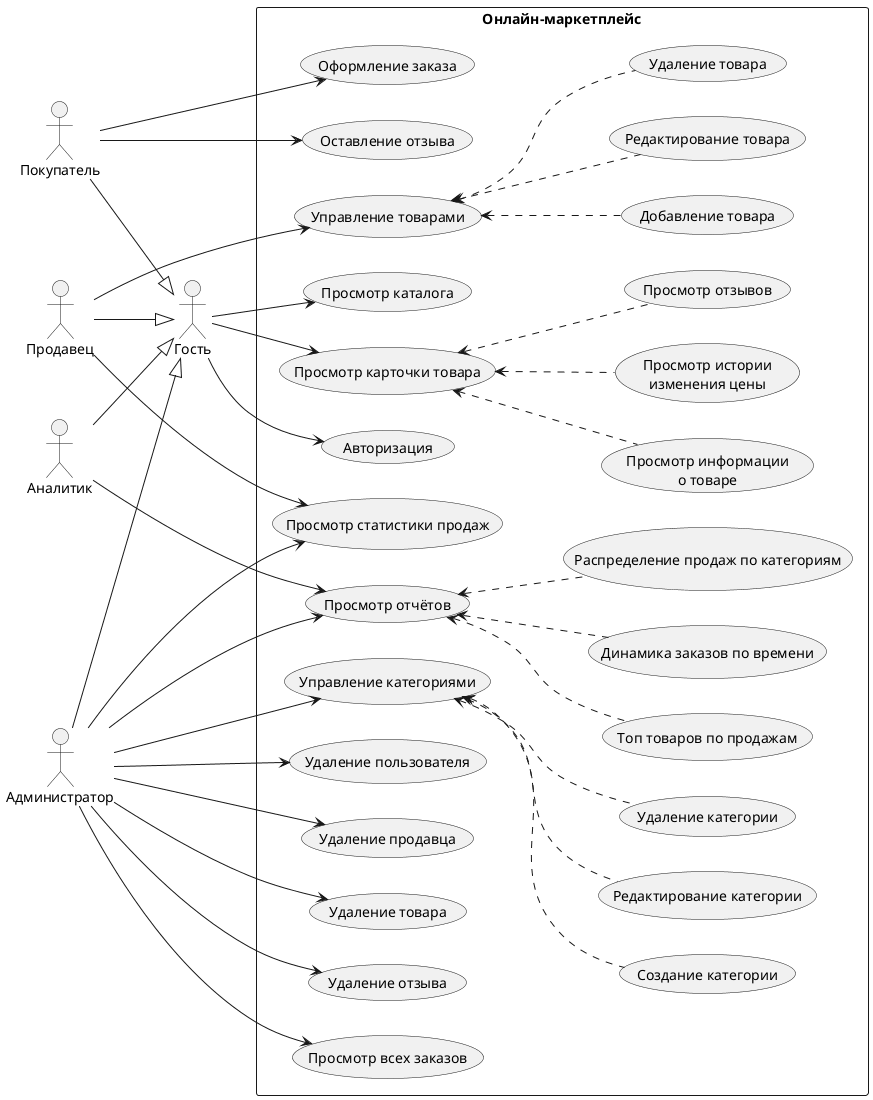
\includegraphics[width=\textwidth]{img/UseCases.png}
    \caption{Диаграмма вариантов использования}
    \label{fig:usecase}
\end{figure}

Каждая авторизованная роль наследует возможности гостя. Администратор, в отличие от покупателя и продавца, не наследует их бизнес-действий, а обладает собственным набором операций, ориентированных на модерацию и контроль данных платформы.


% !TEX root = ../../report.tex

\section{Описание данных и структур}

На основе анализа предметной области и сформулированных требований выделены следующие сущности:

\begin{itemize}
    \item пользователь;
    \item продавец;
    \item товар;
    \item категория;
    \item заказ;
    \item позиция заказа;
    \item отзыв;
    \item адрес доставки;
    \item история изменения цен.
\end{itemize}

Дополнительно выделена связующая сущность <<товар--категория>> для представления связи <<многие ко многим>> между товарами и категориями. Таким образом, общее число сущностей составляет 10.

Сведения о признаках сущностей приведены в таблице~\ref{tbl:entities}.

\begin{table}[H]
    \caption{Сведения о сущностях предметной области}
    \label{tbl:entities}
    \begin{tabular}{|l|l|}
        \hline
        \textbf{Сущность} & \textbf{Данные} \\ \hline
        Пользователь & \makecell[l]{Идентификатор, Email,\\ Данные авторизации, Полное имя,\\ Телефон, Роль} \\ \hline
        Продавец & \makecell[l]{Идентификатор, Пользователь,\\ Название компании, Описание, Рейтинг} \\ \hline
        Товар & \makecell[l]{Идентификатор, Продавец, Название,\\ Описание, Цена, Количество на складе,\\ Количество в резерве, Рейтинг} \\ \hline
        Категория & \makecell[l]{Идентификатор, Родительская категория,\\ Название, Описание} \\ \hline
        Заказ & \makecell[l]{Идентификатор, Покупатель,\\ Продавец для оформленного заказа,\\ Адрес доставки для оформленного заказа,\\ Статус, Итоговая сумма} \\ \hline
        Позиция заказа & \makecell[l]{Идентификатор, Заказ, Товар,\\ Количество, Цена на момент покупки} \\ \hline
        Отзыв & \makecell[l]{Идентификатор, Пользователь, Товар,\\ Оценка (1--5), Комментарий} \\ \hline
        Адрес доставки & \makecell[l]{Идентификатор, Пользователь, Город,\\ Улица, Дом, Квартира, Индекс,\\ Признак основного} \\ \hline
        История цен & \makecell[l]{Идентификатор, Товар, Старая цена,\\ Новая цена, Дата изменения, Кто изменил} \\ \hline
    \end{tabular}
\end{table}

Между сущностями установлены следующие связи:

\begin{itemize}
    \item пользователь~--- продавец: один к нулю или одному (профиль продавца связывается только с учётной записью, имеющей роль продавца);
    \item пользователь~--- заказ: один ко многим (покупатель оформляет несколько заказов);
    \item пользователь~--- адрес: один ко многим;
    \item пользователь~--- отзыв: один ко многим;
    \item продавец~--- товар: один ко многим;
    \item продавец~--- оформленный заказ: один ко многим;
    \item товар~--- категория: многие ко многим (через связующую сущность);
    \item товар~--- отзыв: один ко многим;
    \item товар~--- история цен: один ко многим;
    \item категория~--- категория: один ко многим (иерархия через ссылку на родительскую категорию);
    \item заказ~--- позиция заказа: один ко многим;
    \item оформленный заказ~--- адрес: многие к одному;
    \item позиция заказа~--- товар: многие к одному.
\end{itemize}

На рисунке~\ref{fig:ER} приведена концептуальная диаграмма сущность-связь в нотации Чена.

\begin{figure}[H]
    \centering
    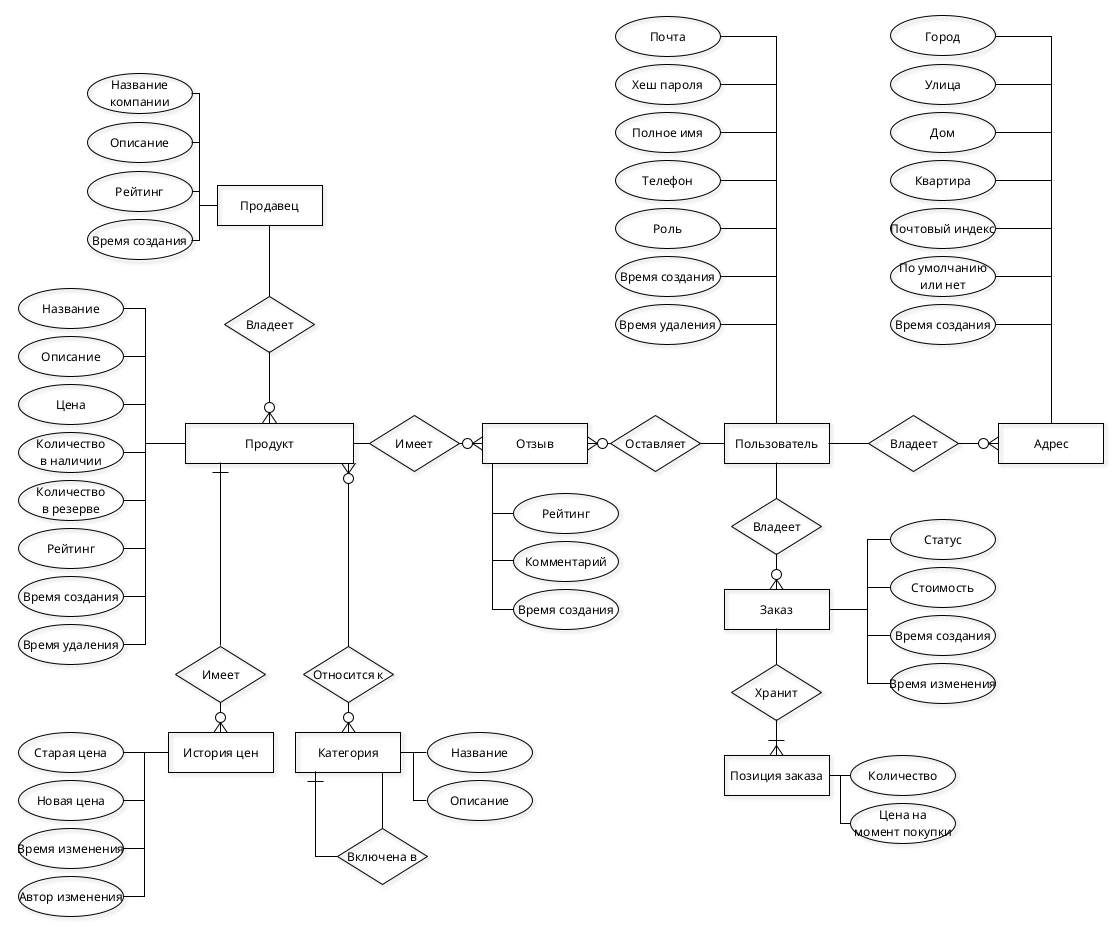
\includegraphics[width=\textwidth]{img/ER_Chen.png}
    \caption{Диаграмма сущность-связь в нотации Чена}
    \label{fig:ER}
\end{figure}

Бизнес-правило <<корзина как черновик заказа>> позволяет не выделять корзину в самостоятельную сущность. Черновик заказа не связан с адресом доставки и продавцом, а при оформлении разделяется на несколько заказов --- по одному на каждого продавца. В момент оформления фиксируется цена товара для соответствующей позиции заказа.

Для контроля доступного остатка товара учитываются общий остаток у продавца и количество товара, находящееся в резерве по оформленным заказам. Доступное для нового заказа количество определяется как разность общего остатка и зарезервированного количества.

Жизненный цикл заказа включает состояния черновика, ожидания оплаты, оплаты, отгрузки, доставки и отмены. При оформлении заказа товар резервируется. При отмене заказа или истечении срока оплаты резерв освобождается. При отгрузке уменьшается общий складской остаток и соответствующее количество в резерве. Отмена заказа допускается до отгрузки.

Для формирования аналитической отчётности необходимы показатели по продавцу за временной интервал: количество заказов, общая выручка, средний чек и наименование самого продаваемого товара.


% !TEX root = ../../report.tex

\section{Анализ моделей баз данных}

Для выбора модели хранения данных рассмотрены три группы моделей: дореляционные, реляционные и постреляционные~\cite{db_models}. Сравнение выполняется по признакам, связанным с проектируемой системой: фиксированность схемы, наличие стандартного языка запросов, возможность хранения неструктурированных данных и поддержка целостности.

Дореляционные модели используют иерархические или сетевые связи между записями с жёстко заданной схемой и структурированными записями. Такая организация усложняет изменение связей и выполнение декларативных запросов к данным~\cite{db_models}. Постреляционные модели расширяют реляционный подход средствами хранения составных и полуструктурированных данных. Для текущей задачи такие возможности не являются основными, так как каталог, заказы, пользователи и отзывы имеют заранее определённые атрибуты и связи.

Реляционная модель представляет данные в виде отношений, поддерживает ключи, внешние связи и стандартный язык запросов~\cite{db_models, relation_model}. Эти свойства соответствуют требованиям проектируемой системы: требуется хранить связанные сущности, контролировать целостность данных и разграничивать доступ к ним.

Сравнение рассмотренных групп моделей представлено в таблице~\ref{tbl:model_comparison}.

\begin{table}[H]
    \caption{Сравнение моделей БД}
    \label{tbl:model_comparison}
    \centering
    \begin{tabular}{|l|l|l|l|}
        \hline
        \multicolumn{1}{|c|}{\multirow{2}{*}{\textbf{Критерий}}} & \multicolumn{3}{c|}{\textbf{Модель}} \\ \cline{2-4}
        \multicolumn{1}{|c|}{} & \makecell[l]{Дореля-\\ционная} & \makecell[l]{Реля-\\ционная} & \makecell[l]{Постреля-\\ционная} \\ \hline
        \makecell[l]{Фиксированная\\схема данных} & Да & Да & Частично \\ \hline
        \makecell[l]{Стандартный\\язык запросов} & Нет & Да & Да \\ \hline
        \makecell[l]{Хранение неструкту-\\рированных данных} & Нет & Нет & Да \\ \hline
        \makecell[l]{Обеспечение\\целостности данных} & Частично & Да & Частично \\ \hline
    \end{tabular}
\end{table}

Для проектируемой системы выбрана \textbf{реляционная модель} базы данных. Она соответствует структуре данных онлайн-маркетплейса и позволяет описать связи между товарами, заказами, пользователями, отзывами и категориями средствами ограничений целостности.



% !TEX root = ../report.tex

\chapter{Конструкторская часть}

В данном разделе производится формализация сущностей базы данных, описываются столбцы таблиц и ограничения целостности. Устанавливается ролевая модель доступа на уровне СУБД, проектируются триггеры и хранимая функция. Проводится проверка соответствия спроектированной базы данных третьей нормальной форме.

% !TEX root = ../../report.tex

\section{Описание сущностей базы данных}

В соответствии с таблицей~\ref{tbl:entities}, описывающей сущности предметной области, выделяются следующие таблицы:

\begin{itemize}
    \item users --- таблица пользователей;
    \item sellers --- таблица продавцов;
    \item products --- таблица товаров;
    \item categories --- таблица категорий;
    \item product\_categories --- таблица связей товаров и категорий;
    \item addresses --- таблица адресов доставки;
    \item orders --- таблица заказов;
    \item order\_items --- таблица позиций заказов;
    \item reviews --- таблица отзывов;
    \item product\_price\_history --- таблица истории изменения цен.
\end{itemize}

В таблицах~\ref{tbl:t_users}--\ref{tbl:t_price_history} приведены столбцы и их ограничения для каждой из перечисленных таблиц.

\begin{table}[H]
    \caption{Описание столбцов таблицы users}
    \label{tbl:t_users}
    \begin{tabular}[]{|c|c|c|c|}
        \hline
        \textbf{Столбец} & \textbf{Тип данных} & \textbf{Ограничения} & \textbf{Описание} \\ \hline
        id & BIGSERIAL & \makecell{NOT NULL \\ PRIMARY KEY} & идентификатор \\ \hline
        email & VARCHAR(255) & \makecell{NOT NULL \\ UNIQUE} & электронная почта \\ \hline
        password\_hash & VARCHAR(255) & NOT NULL & хеш пароля \\ \hline
        full\_name & VARCHAR(255) & NOT NULL & полное имя \\ \hline
        phone & VARCHAR(20) & --- & номер телефона \\ \hline
        role & VARCHAR(20) & \makecell{NOT NULL \\ CHECK} & \makecell{роль: buyer, seller,\\admin, analyst} \\ \hline
        created\_at & TIMESTAMPTZ & \makecell{NOT NULL \\ DEFAULT now()} & дата создания \\ \hline
        deleted\_at & TIMESTAMPTZ & --- & \makecell{дата мягкого\\удаления} \\ \hline
    \end{tabular}
\end{table}

\begin{table}[H]
    \caption{Описание столбцов таблицы sellers}
    \label{tbl:t_sellers}
    \begin{tabular}[]{|c|c|c|c|}
        \hline
        \textbf{Столбец} & \textbf{Тип данных} & \textbf{Ограничения} & \textbf{Описание} \\ \hline
        id & BIGSERIAL & \makecell{NOT NULL \\ PRIMARY KEY} & идентификатор \\ \hline
        user\_id & BIGINT & \makecell{NOT NULL \\ UNIQUE \\ FOREIGN KEY} & \makecell{ссылка на\\пользователя} \\ \hline
        company\_name & VARCHAR(255) & NOT NULL & название компании \\ \hline
        description & TEXT & --- & описание \\ \hline
        rating & NUMERIC(3,2) & --- & \makecell{рейтинг\\(пересчитывается\\триггером)} \\ \hline
        created\_at & TIMESTAMPTZ & \makecell{NOT NULL \\ DEFAULT now()} & дата создания \\ \hline
    \end{tabular}
\end{table}

\begin{table}[H]
    \caption{Описание столбцов таблицы products}
    \label{tbl:t_products}
    \begin{tabular}[]{|c|c|c|c|}
        \hline
        \textbf{Столбец} & \textbf{Тип данных} & \textbf{Ограничения} & \textbf{Описание} \\ \hline
        id & BIGSERIAL & \makecell{NOT NULL \\ PRIMARY KEY} & идентификатор \\ \hline
        seller\_id & BIGINT & \makecell{NOT NULL \\ FOREIGN KEY} & \makecell{ссылка на\\продавца} \\ \hline
        name & VARCHAR(255) & NOT NULL & название товара \\ \hline
        description & TEXT & --- & описание \\ \hline
        price & NUMERIC(12,2) & \makecell{NOT NULL \\ CHECK $> 0$} & цена \\ \hline
        stock\_quantity & INTEGER & \makecell{NOT NULL \\ CHECK $\geq 0$ \\ DEFAULT 0} & \makecell{количество\\на складе} \\ \hline
        reserved\_quantity & INTEGER & \makecell{NOT NULL \\ CHECK $\geq 0$ \\ DEFAULT 0 \\ CHECK $\leq$\\stock\_quantity} & \makecell{количество\\в резерве} \\ \hline
        rating & NUMERIC(3,2) & --- & \makecell{рейтинг\\(пересчитывается\\триггером)} \\ \hline
        created\_at & TIMESTAMPTZ & \makecell{NOT NULL \\ DEFAULT now()} & дата создания \\ \hline
        deleted\_at & TIMESTAMPTZ & --- & \makecell{дата мягкого\\удаления} \\ \hline
    \end{tabular}
\end{table}

\begin{table}[H]
    \caption{Описание столбцов таблицы categories}
    \label{tbl:t_categories}
    \begin{tabular}[]{|c|c|c|c|}
        \hline
        \textbf{Столбец} & \textbf{Тип данных} & \textbf{Ограничения} & \textbf{Описание} \\ \hline
        id & BIGSERIAL & \makecell{NOT NULL \\ PRIMARY KEY} & идентификатор \\ \hline
        parent\_id & BIGINT & FOREIGN KEY & \makecell{ссылка на\\родительскую\\категорию} \\ \hline
        name & VARCHAR(255) & \makecell{NOT NULL \\ UNIQUE} & название категории \\ \hline
        description & TEXT & --- & описание \\ \hline
    \end{tabular}
\end{table}

\begin{table}[H]
    \caption{Описание столбцов таблицы product\_categories}
    \label{tbl:t_product_categories}
    \begin{tabular}[]{|c|c|c|c|}
        \hline
        \textbf{Столбец} & \textbf{Тип данных} & \textbf{Ограничения} & \textbf{Описание} \\ \hline
        product\_id & BIGINT & \makecell{NOT NULL \\ FOREIGN KEY} & \makecell{ссылка на\\товар} \\ \hline
        category\_id & BIGINT & \makecell{NOT NULL \\ FOREIGN KEY} & \makecell{ссылка на\\категорию} \\ \hline
        \multicolumn{4}{|c|}{PRIMARY KEY (product\_id, category\_id)} \\ \hline
    \end{tabular}
\end{table}

\begin{table}[H]
    \caption{Описание столбцов таблицы addresses}
    \label{tbl:t_addresses}
    \begin{tabular}[]{|c|c|c|c|}
        \hline
        \textbf{Столбец} & \textbf{Тип данных} & \textbf{Ограничения} & \textbf{Описание} \\ \hline
        id & BIGSERIAL & \makecell{NOT NULL \\ PRIMARY KEY} & идентификатор \\ \hline
        user\_id & BIGINT & \makecell{NOT NULL \\ FOREIGN KEY} & \makecell{ссылка на\\пользователя} \\ \hline
        city & VARCHAR(100) & NOT NULL & город \\ \hline
        street & VARCHAR(255) & NOT NULL & улица \\ \hline
        house & VARCHAR(20) & NOT NULL & дом \\ \hline
        apartment & VARCHAR(20) & --- & квартира \\ \hline
        zip\_code & VARCHAR(20) & NOT NULL & почтовый индекс \\ \hline
        is\_default & BOOLEAN & \makecell{NOT NULL \\ DEFAULT false} & \makecell{признак основного\\адреса} \\ \hline
        created\_at & TIMESTAMPTZ & \makecell{NOT NULL \\ DEFAULT now()} & дата создания \\ \hline
    \end{tabular}
\end{table}

\begin{table}[H]
    \caption{Описание столбцов таблицы orders}
    \label{tbl:t_orders}
    \begin{tabular}[]{|c|c|c|c|}
        \hline
        \textbf{Столбец} & \textbf{Тип данных} & \textbf{Ограничения} & \textbf{Описание} \\ \hline
        id & BIGSERIAL & \makecell{NOT NULL \\ PRIMARY KEY} & идентификатор \\ \hline
        user\_id & BIGINT & \makecell{NOT NULL \\ FOREIGN KEY} & \makecell{ссылка на\\покупателя} \\ \hline
        seller\_id & BIGINT & \makecell{FOREIGN KEY \\ (nullable)} & \makecell{ссылка на продавца\\(заполняется при\\оформлении)} \\ \hline
        address\_id & BIGINT & \makecell{FOREIGN KEY \\ (nullable)} & \makecell{ссылка на адрес\\(null для\\корзины-черновика)} \\ \hline
        status & VARCHAR(30) & \makecell{NOT NULL \\ CHECK} & \makecell{статус: draft,\\pending, paid,\\shipped, delivered,\\cancelled} \\ \hline
        total\_amount & NUMERIC(12,2) & \makecell{NOT NULL \\ CHECK $\geq 0$} & итоговая сумма \\ \hline
        created\_at & TIMESTAMPTZ & \makecell{NOT NULL \\ DEFAULT now()} & дата создания \\ \hline
        updated\_at & TIMESTAMPTZ & \makecell{NOT NULL \\ DEFAULT now()} & дата обновления \\ \hline
    \end{tabular}
\end{table}

\begin{table}[H]
    \caption{Описание столбцов таблицы order\_items}
    \label{tbl:t_order_items}
    \begin{tabular}[]{|c|c|c|c|}
        \hline
        \textbf{Столбец} & \textbf{Тип данных} & \textbf{Ограничения} & \textbf{Описание} \\ \hline
        id & BIGSERIAL & \makecell{NOT NULL \\ PRIMARY KEY} & идентификатор \\ \hline
        order\_id & BIGINT & \makecell{NOT NULL \\ FOREIGN KEY} & ссылка на заказ \\ \hline
        product\_id & BIGINT & \makecell{NOT NULL \\ FOREIGN KEY} & ссылка на товар \\ \hline
        quantity & INTEGER & \makecell{NOT NULL \\ CHECK $> 0$} & количество \\ \hline
        price\_at\_purchase & NUMERIC(12,2) & \makecell{NOT NULL \\ CHECK $> 0$} & \makecell{цена на момент\\покупки} \\ \hline
        \multicolumn{4}{|c|}{UNIQUE (order\_id, product\_id)} \\ \hline
    \end{tabular}
\end{table}

\begin{table}[H]
    \caption{Описание столбцов таблицы reviews}
    \label{tbl:t_reviews}
    \begin{tabular}[]{|c|c|c|c|}
        \hline
        \textbf{Столбец} & \textbf{Тип данных} & \textbf{Ограничения} & \textbf{Описание} \\ \hline
        id & BIGSERIAL & \makecell{NOT NULL \\ PRIMARY KEY} & идентификатор \\ \hline
        user\_id & BIGINT & \makecell{NOT NULL \\ FOREIGN KEY} & \makecell{ссылка на\\пользователя} \\ \hline
        product\_id & BIGINT & \makecell{NOT NULL \\ FOREIGN KEY} & ссылка на товар \\ \hline
        rating & SMALLINT & \makecell{NOT NULL \\ CHECK 1..5} & оценка от 1 до 5 \\ \hline
        comment & TEXT & --- & текст отзыва \\ \hline
        created\_at & TIMESTAMPTZ & \makecell{NOT NULL \\ DEFAULT now()} & дата создания \\ \hline
        \multicolumn{4}{|c|}{UNIQUE (user\_id, product\_id)} \\ \hline
    \end{tabular}
\end{table}

\begin{table}[H]
    \caption{Описание столбцов таблицы product\_price\_history}
    \label{tbl:t_price_history}
    \begin{tabular}[]{|c|c|c|c|}
        \hline
        \textbf{Столбец} & \textbf{Тип данных} & \textbf{Ограничения} & \textbf{Описание} \\ \hline
        id & BIGSERIAL & \makecell{NOT NULL \\ PRIMARY KEY} & идентификатор \\ \hline
        product\_id & BIGINT & \makecell{NOT NULL \\ FOREIGN KEY} & ссылка на товар \\ \hline
        old\_price & NUMERIC(12,2) & NOT NULL & старая цена \\ \hline
        new\_price & NUMERIC(12,2) & NOT NULL & новая цена \\ \hline
        changed\_at & TIMESTAMPTZ & \makecell{NOT NULL \\ DEFAULT now()} & дата изменения \\ \hline
        changed\_by & TEXT & \makecell{NOT NULL \\ DEFAULT\\current\_user} & \makecell{инициатор\\изменения} \\ \hline
    \end{tabular}
\end{table}

Помимо первичных ключей и ограничений уникальности, для оптимизации запросов создаются дополнительные индексы. Перечень индексов приведён в таблице~\ref{tbl:indexes}.

\begin{table}[H]
    \caption{Индексы базы данных}
    \label{tbl:indexes}
    \begin{tabular}{|l|l|l|}
        \hline
        \textbf{Индекс} & \textbf{Столбцы} & \textbf{Назначение} \\ \hline
        \makecell[l]{idx\_products\_\\seller\_id} & \makecell[l]{products\\(seller\_id)} & \makecell[l]{выборка товаров\\продавца} \\ \hline
        \makecell[l]{idx\_orders\_\\user\_id} & \makecell[l]{orders\\(user\_id)} & \makecell[l]{выборка заказов\\покупателя} \\ \hline
        \makecell[l]{ux\_orders\_one\_\\draft\_per\_user} & \makecell[l]{orders\\(user\_id)\\WHERE status = 'draft'} & \makecell[l]{единственная\\корзина покупателя} \\ \hline
        \makecell[l]{idx\_orders\_\\status\_created\_at} & \makecell[l]{orders\\(status, created\_at)} & \makecell[l]{фильтрация заказов\\по статусу и дате} \\ \hline
        \makecell[l]{idx\_product\_\\categories\_\\category\_id} & \makecell[l]{product\_categories\\(category\_id)} & \makecell[l]{выборка товаров\\по категории} \\ \hline
        \makecell[l]{idx\_reviews\_\\product\_id} & \makecell[l]{reviews\\(product\_id)} & \makecell[l]{выборка отзывов\\на товар} \\ \hline
        \makecell[l]{idx\_products\_\\id\_not\_deleted} & \makecell[l]{products (id)\\WHERE deleted\_at\\IS NULL} & \makecell[l]{частичный индекс:\\только активные\\товары} \\ \hline
        \makecell[l]{idx\_users\_\\id\_not\_deleted} & \makecell[l]{users (id)\\WHERE deleted\_at\\IS NULL} & \makecell[l]{частичный индекс:\\только активные\\пользователи} \\ \hline
        \makecell[l]{idx\_products\_\\price} & \makecell[l]{products\\(price)} & \makecell[l]{сортировка и\\фильтрация по цене} \\ \hline
    \end{tabular}
\end{table}

Частичные индексы (\texttt{WHERE deleted\_at IS NULL}) обеспечивают эффективный поиск только среди активных записей, исключая мягко удалённые строки из индексного дерева.

\clearpage


% !TEX root = ../../report.tex

\section{Ролевая модель}

Ролевая модель используется для разграничения доступа к таблицам базы данных на уровне СУБД. Каждой роли назначается набор привилегий, определяющий допустимые операции.

В аналитической части были определены пять ролей пользователей системы. На уровне СУБД проектируются четыре роли, соответствующие авторизованным пользователям. Роль гостя не выделяется как отдельная роль СУБД, поскольку действия гостя ограничиваются просмотром общедоступных данных и авторизацией. Просмотр гостем общедоступных данных соответствует чтению каталога, карточек продавцов, отзывов и истории цен.

Описание привилегий каждой роли приведено ниже.

\textbf{marketplace\_buyer} --- роль покупателя:
\begin{itemize}
    \item чтение таблиц products, sellers, categories, product\_categories, reviews, product\_price\_history --- просмотр каталога, карточек товаров, продавцов, отзывов и истории цен;
    \item управление таблицами addresses, reviews, orders, order\_items --- работа с адресами, отзывами, заказами и позициями заказа.
\end{itemize}

\textbf{marketplace\_seller} --- роль продавца:
\begin{itemize}
    \item управление таблицами sellers, products, product\_categories --- работа с профилем продавца, товарами и их категориями;
    \item чтение таблиц categories, reviews, product\_price\_history --- просмотр категорий, отзывов и истории цен;
    \item чтение таблиц orders и order\_items, обновление таблицы orders --- просмотр заказов продавца и фиксация статусов отгрузки и доставки.
\end{itemize}

\textbf{marketplace\_admin} --- роль администратора:
\begin{itemize}
    \item управление всеми таблицами --- полный доступ к данным.
\end{itemize}

\textbf{marketplace\_analyst} --- роль аналитика:
\begin{itemize}
    \item чтение всех таблиц --- доступ к данным без возможности модификации.
\end{itemize}

Сводная таблица привилегий ролей приведена в таблице~\ref{tbl:role_matrix}.

\begin{table}[H]
    \caption{Матрица привилегий ролей}
    \label{tbl:role_matrix}
    \begin{tabular}{|l|c|c|c|c|}
        \hline
        \textbf{Таблица} & \textbf{buyer} & \textbf{seller} & \textbf{admin} & \textbf{analyst} \\ \hline
        users & --- & --- & CRUD & R \\ \hline
        sellers & R & CRUD & CRUD & R \\ \hline
        products & R & CRUD & CRUD & R \\ \hline
        categories & R & R & CRUD & R \\ \hline
        product\_categories & R & CRUD & CRUD & R \\ \hline
        addresses & CRUD & --- & CRUD & R \\ \hline
        orders & CRUD & RU & CRUD & R \\ \hline
        order\_items & CRUD & R & CRUD & R \\ \hline
        reviews & CRUD & R & CRUD & R \\ \hline
        product\_price\_history & R & R & CRUD & R \\ \hline
    \end{tabular}
\end{table}

Обозначения в таблице: C --- CREATE (INSERT), R --- READ (SELECT), U --- UPDATE, D --- DELETE. Прочерк означает отсутствие доступа к данной таблице.

Матрица описывает привилегии на уровне таблиц. Правила принадлежности отдельных записей соответствуют ограничениям предметной области: продавец работает со своим профилем, своими товарами, категориями своих товаров и заказами, покупатель --- со своими заказами, позициями заказа, адресами и отзывами. История цен формируется триггером; покупатель и продавец имеют доступ только на чтение этой таблицы.

Полный доступ администратора в матрице относится к уровню СУБД. Пользовательские сценарии администратора остаются заданными в аналитической части.


% !TEX root = ../../report.tex

\section{Триггеры и хранимая функция}

В проектируемой базе данных предусмотрены два триггера и одна хранимая функция.

\subsection{Триггер аудита изменений цен}

Триггер \texttt{catch\_price\_change} активируется после обновления столбца \texttt{price} в таблице \texttt{products}. Условие срабатывания --- старое значение цены отличается от нового. При срабатывании вызывается функция аудита цены, которая вставляет запись в таблицу \texttt{product\_price\_history}, содержащую:

\begin{itemize}
    \item идентификатор товара;
    \item старую и новую цену;
    \item метку времени изменения;
    \item имя пользователя, инициировавшего изменение.
\end{itemize}

Схема алгоритма триггера приведена на рисунке~\ref{fig:trigger_price}.

\begin{figure}[H]
    \centering
    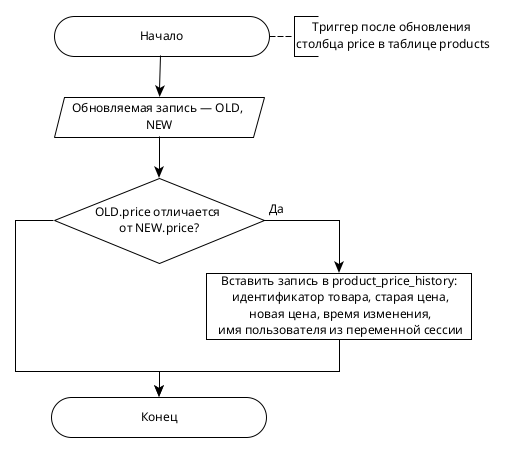
\includegraphics[width=0.7\textwidth]{img/trigger_catch_price_change.png}
    \caption{Схема алгоритма триггера аудита изменений цен}
    \label{fig:trigger_price}
\end{figure}

Триггер обеспечивает автоматическое формирование журнала изменения цен.

\subsection{Триггер пересчёта рейтингов}

Триггер \texttt{update\_ratings\_on\_review} активируется после вставки новой записи, обновления столбца \texttt{rating} или удаления записи в таблице \texttt{reviews}. Вызываемая функция \texttt{update\_product\_and\_seller\_rating} выполняет каскадный пересчёт:

\begin{enumerate}
    \item определяется идентификатор затронутого товара;
    \item рейтинг товара обновляется как среднее арифметическое оценок всех отзывов на данный товар (\texttt{AVG(rating)});
    \item по идентификатору продавца, полученному из обновлённой записи товара, пересчитывается рейтинг продавца как среднее арифметическое рейтингов всех его неудалённых товаров, имеющих хотя бы один отзыв.
\end{enumerate}

Схема алгоритма триггера приведена на рисунке~\ref{fig:trigger_rating}.

\begin{figure}[H]
    \centering
    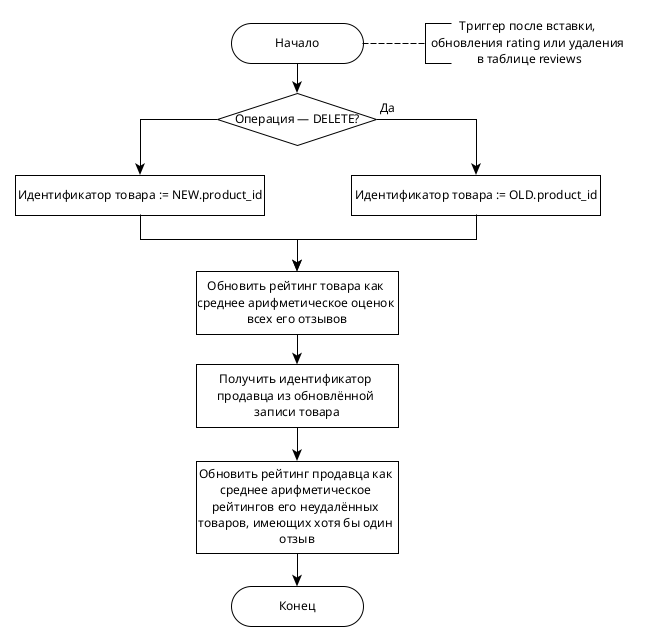
\includegraphics[width=0.7\textwidth]{img/trigger_update_ratings_on_review.png}
    \caption{Схема алгоритма триггера пересчёта рейтингов}
    \label{fig:trigger_rating}
\end{figure}

Такой подход поддерживает согласованность рейтингов: при добавлении, изменении или удалении отзыва автоматически обновляются рейтинги товара и продавца.

\subsection{Хранимая функция статистики продавца}

Функция \texttt{get\_seller\_statistics} принимает три параметра: идентификатор продавца (\texttt{p\_seller\_id}), начальную (\texttt{p\_date\_from}) и конечную (\texttt{p\_date\_to}) даты периода. Возвращает таблицу из четырёх столбцов:

\begin{itemize}
    \item \texttt{total\_orders} --- количество уникальных заказов;
    \item \texttt{total\_revenue} --- суммарная выручка;
    \item \texttt{avg\_order\_value} --- средний чек;
    \item \texttt{top\_product\_name} --- наименование самого продаваемого товара по количеству проданных единиц.
\end{itemize}

Функция объединяет данные таблиц \texttt{orders}, \texttt{order\_items} и \texttt{products} по идентификатору продавца и заданному временному интервалу. В расчёт включаются только заказы со статусами \texttt{paid}, \texttt{shipped} и \texttt{delivered}, что исключает из статистики неоплаченные и отменённые заказы.

Выручка рассчитывается как сумма произведений количества единиц товара на цену в момент покупки, что обеспечивает корректность подсчёта при наличии изменений цен. Средний чек вычисляется путём деления выручки на количество уникальных заказов.

Схема алгоритма функции приведена на рисунке~\ref{fig:function_stats}.

\begin{figure}[H]
    \centering
    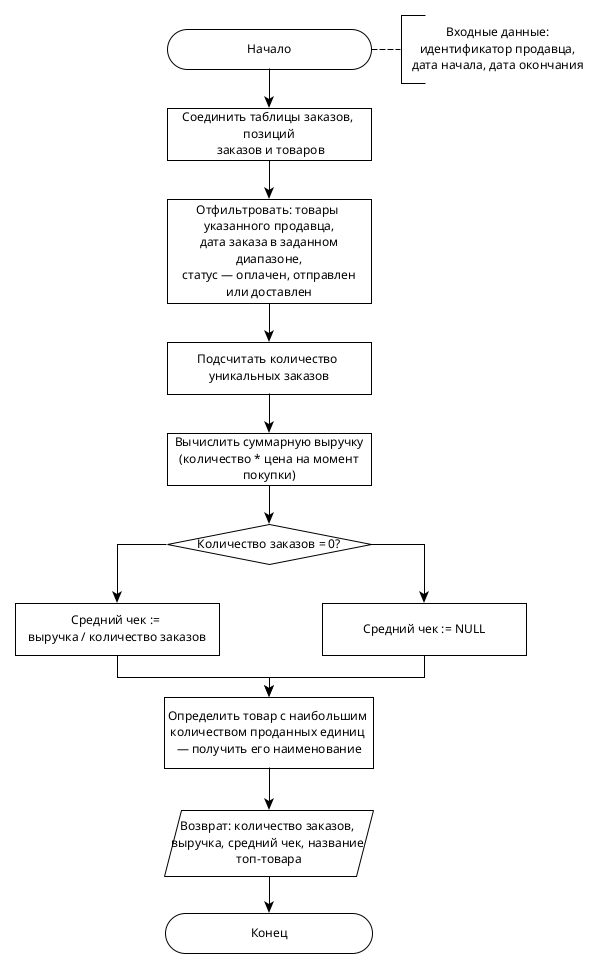
\includegraphics[width=0.7\textwidth]{img/function_get_seller_statistics.png}
    \caption{Схема алгоритма хранимой функции статистики продавца}
    \label{fig:function_stats}
\end{figure}


% !TEX root = ../../report.tex

\section{Проверка соответствия третьей нормальной форме}

Согласно требованиям к курсовой работе, спроектированная база данных должна находиться в третьей нормальной форме (3НФ). Отношение находится в 3НФ, если оно находится во второй нормальной форме и ни один неключевой атрибут не зависит транзитивно от первичного ключа~\cite{db_models}.

Проверка выполняется последовательно для каждой нормальной формы.

\subsection*{Первая нормальная форма (1НФ)}

Отношение находится в 1НФ, если все атрибуты содержат атомарные (неделимые) значения. В спроектированной базе данных это условие выполняется:

\begin{itemize}
    \item адрес доставки разделён на атомарные компоненты: \texttt{city}, \texttt{street}, \texttt{house}, \texttt{apartment}, \texttt{zip\_code};
    \item связь <<многие ко многим>> между товарами и категориями вынесена в отдельную таблицу \texttt{product\_categories};
    \item все остальные атрибуты содержат скалярные значения (строки, числа, даты, логические значения).
\end{itemize}

\subsection*{Вторая нормальная форма (2НФ)}

Отношение находится в 2НФ, если оно находится в 1НФ и каждый неключевой атрибут полностью функционально зависит от первичного ключа (отсутствуют частичные зависимости).

В большинстве таблиц первичным ключом является суррогатный идентификатор \texttt{id} (одноатрибутный ключ), при котором частичные зависимости невозможны по определению.

Единственная таблица с составным первичным ключом --- \texttt{product\_cate\-gories}. Ключ состоит из двух внешних ключей: \texttt{product\_id} и \texttt{category\_id}. Таблица не содержит неключевых атрибутов, следовательно, условие 2НФ выполняется тривиально.

\subsection*{Третья нормальная форма (3НФ)}

Отношение находится в 3НФ, если оно находится в 2НФ и не содержит транзитивных зависимостей неключевых атрибутов от первичного ключа.

Рассмотрим таблицы, в которых потенциально могут возникнуть транзитивные зависимости:

\begin{itemize}
    \item \textbf{orders}: атрибуты \texttt{user\_id}, \texttt{seller\_id} и \texttt{address\_id} являются внешними ключами, а не производными данными. Атрибут \texttt{total\_amount} может рассматриваться как вычисляемый (сумма позиций), однако хранится денормализованно для оптимизации выборок и фиксируется на момент оформления заказа;
    \item \textbf{products}: атрибут \texttt{rating} пересчитывается триггером на основе таблицы \texttt{reviews}. Формально это производное значение, хранимое для сокращения повторных расчётов рейтинга по отзывам. Атрибут \texttt{reserved\_quantity} хранит операционное состояние резерва товара и ограничивается условием \texttt{reserved\_quantity} $\leq$ \texttt{stock\_quantity};
    \item \textbf{sellers}: аналогично, \texttt{rating} пересчитывается триггером из рейтингов товаров.
\end{itemize}

Атрибуты \texttt{rating} в таблицах \texttt{products} и \texttt{sellers}, а также \texttt{total\_amount} в таблице \texttt{orders} представляют собой контролируемую денормализацию. Их значения должны поддерживаться в согласованном состоянии правилами проектируемой базы данных и правилами обработки заказов. Все остальные неключевые атрибуты зависят только от первичного ключа своей таблицы.

Таким образом, спроектированная база данных находится в третьей нормальной форме с обоснованной денормализацией вычисляемых агрегатов.



% !TEX root = ../report.tex

\chapter{Технологическая часть}

В данном разделе описывается реализация базы данных и программного интерфейса доступа к ней. Рассматриваются средства реализации, порядок применения миграций, реализованные ограничения целостности, роли СУБД, триггеры, хранимая функция, Redis-кэширование и REST-интерфейс.

\section{Выбор средств реализации}

Для реализации базы данных используется PostgreSQL 16. PostgreSQL относится к реляционным СУБД и поддерживает транзакции, внешние ключи, ограничения целостности, частичные индексы, пользовательские роли, триггеры и хранимые функции на языке PL/pgSQL~\cite{postgresql_doc}. Эти возможности соответствуют требованиям проектируемой системы: данные маркетплейса имеют выраженную табличную структуру, а часть правил целостности должна выполняться непосредственно на уровне базы данных.

Выбор СУБД выполнен по критериям, связанным с реализуемой схемой. В качестве альтернатив рассматривались PostgreSQL, MySQL и SQLite~\cite{postgresql_doc,mysql_doc,sqlite_doc}. Сравнение приведено в таблице~\ref{tbl:dbms_compare}.

\begin{table}[H]
    \caption{Сравнение СУБД по требованиям реализации}
    \label{tbl:dbms_compare}
    \begin{tabular}{|p{0.36\textwidth}|c|c|c|}
        \hline
        \textbf{Критерий} & \textbf{PostgreSQL} & \textbf{MySQL} & \textbf{SQLite} \\ \hline
        Серверный многопользовательский режим & да & да & нет \\ \hline
        Роли и привилегии на уровне СУБД & да & да & нет \\ \hline
        Хранимые функции с табличным результатом & да & да & нет \\ \hline
        Частичные индексы & да & нет & да \\ \hline
        Статическая типизация столбцов (\texttt{NUMERIC}, \texttt{TIMESTAMP}) & да & да & нет \\ \hline
        Поддержка внешних ключей и транзакций & да & да & да \\ \hline
    \end{tabular}
\end{table}

По результатам сравнения PostgreSQL покрывает все перечисленные требования. В реализации используются роли СУБД, частичные индексы, триггеры и функция, возвращающая табличный результат. Поэтому выбрана СУБД PostgreSQL.

Серверное приложение реализовано на языке Go. Язык используется для реализации HTTP-интерфейса, бизнес-операций, транзакционных сценариев и взаимодействия с PostgreSQL и Redis. В проекте используется Go версии 1.25.0 (директива \texttt{go 1.25.0} в \texttt{go.mod})~\cite{go_doc}. Для работы с PostgreSQL используется драйвер \texttt{pgx/v5}, для маршрутизации HTTP-запросов --- библиотека \texttt{chi}, для построения SQL-запросов --- библиотека \texttt{squirrel}.

Миграции схемы выполняются утилитой \texttt{goose}~\cite{goose_doc}. Каждая миграция содержит секции \texttt{Up} и \texttt{Down}, что позволяет воспроизводимо применять и откатывать изменения схемы. Такой подход фиксирует порядок создания таблиц, ограничений, индексов, ролей, триггеров и функций.

Redis используется как in-memory хранилище для кэша часто читаемых данных и для хранения списка отозванных JWT-токенов~\cite{redis_doc}. PostgreSQL остаётся источником истины; Redis используется только как дополнительный слой ускорения чтения и проверки сессий.

В реализации используются PostgreSQL~16.11, Redis~8.6 и Go~1.25.0. Для работы с PostgreSQL применяется драйвер \texttt{pgx/v5}, для маршрутизации HTTP-запросов --- \texttt{chi}, для построения параметризованных SQL-запросов --- \texttt{squirrel}, для применения миграций --- \texttt{goose}.

\section{Реализация базы данных}

Схема базы данных создаётся набором миграций, расположенных в каталоге \texttt{migrations}. Состав миграций приведён в таблице~\ref{tbl:tech_migrations}. Полные SQL-тексты миграций приведены в приложении~А.

\begin{table}[H]
    \caption{Миграции базы данных}
    \label{tbl:tech_migrations}
    \begin{tabular}{|p{0.22\textwidth}|p{0.70\textwidth}|}
        \hline
        \textbf{Группа миграций} & \textbf{Назначение} \\ \hline
        \texttt{001}, \texttt{006}, \texttt{009}--\texttt{012} & создание таблиц и добавление ограничений предметной области: связь заказа с продавцом, резерв товара, адрес доставки, инварианты корзины и изменение уникальности телефона \\ \hline
        \texttt{002} & создание индексов для выборок товаров, заказов, отзывов, категорий и активных записей \\ \hline
        \texttt{003}, \texttt{008} & создание ролей PostgreSQL, назначение привилегий и добавление системных учётных записей \\ \hline
        \texttt{004}, \texttt{005}, \texttt{007} & создание триггера журнала изменения цен, функции статистики продавца и триггера пересчёта рейтингов \\ \hline
    \end{tabular}
\end{table}

Итоговая схема содержит десять таблиц. Таблицы и ограничения были описаны в конструкторской части в таблицах~\ref{tbl:t_users}--\ref{tbl:t_price_history}. В технологической реализации сохраняются следующие группы ограничений:

\begin{itemize}
    \item ограничения домена значений: положительная цена товара, неотрицательное количество товара, допустимый диапазон оценки отзыва, фиксированный набор ролей и статусов заказа;
    \item ограничения ссылочной целостности: связи товара с продавцом, заказа с покупателем, позиции заказа с заказом и товаром, отзыва с пользователем и товаром;
    \item ограничения уникальности: электронная почта пользователя, профиль продавца на пользователя, имя категории, пара заказа и товара в позиции заказа, пара пользователя и товара в отзыве;
    \item частичный уникальный индекс для ограничения одной draft-корзины на покупателя;
    \item проверка \texttt{reserved\_quantity <= stock\_quantity}, исключающая резервирование количества больше доступного остатка.
\end{itemize}

Для мягкого удаления пользователей и товаров используются столбцы \texttt{deleted\_at}. Поиск активных пользователей и товаров поддерживается частичными индексами \texttt{idx\_users\_id\_not\_deleted} и \texttt{idx\_products\_id\_not\_deleted}. Эти индексы включают только строки, у которых \texttt{deleted\_at IS NULL}.

\section{Реализация ролевой модели}

На уровне PostgreSQL реализованы четыре роли:

\begin{itemize}
    \item \texttt{marketplace\_buyer};
    \item \texttt{marketplace\_seller};
    \item \texttt{marketplace\_admin};
    \item \texttt{marketplace\_analyst}.
\end{itemize}

Роли создаются миграцией \texttt{003\_create\_roles.sql}. Привилегии назначаются командами \texttt{GRANT}.

Роль покупателя получает права чтения каталога и категорий, а также права изменения адресов, отзывов, заказов и позиций заказа. Роль продавца получает права управления товарами и чтения заказов, связанных с его товарами. Роль администратора получает полный доступ к таблицам и последовательностям. Роль аналитика получает доступ только на чтение.

Роли PostgreSQL задают технический уровень доступа к объектам БД. Правила принадлежности отдельных строк проверяются в приложении при выполнении пользовательских операций. Например, покупатель работает только со своими адресами, заказами и отзывами, а продавец --- со своим профилем, своими товарами и заказами, относящимися к этим товарам.

\section{Реализация триггеров и хранимой функции}

В базе данных реализованы два триггера и одна хранимая функция. Их назначение соответствует проектным решениям, описанным в конструкторской части.

Триггер \texttt{catch\_price\_change} создаётся миграцией \texttt{004}. Он срабатывает после изменения столбца \texttt{price} в таблице \texttt{products}. Условие \texttt{OLD.price IS DISTINCT FROM NEW.price} исключает запись в журнал при отсутствии фактического изменения цены. При срабатывании триггера функция аудита добавляет строку в таблицу \texttt{product\_price\_history}.

Триггер \texttt{update\_ratings\_on\_review} создаётся миграцией \texttt{007}. Он срабатывает после добавления отзыва, изменения оценки или удаления отзыва. Функция пересчёта рейтингов обновляет рейтинг товара как среднее значение оценок по этому товару. Затем пересчитывается рейтинг продавца как среднее значение рейтингов его активных товаров.

Хранимая функция \texttt{get\_seller\_statistics} создаётся миграцией \texttt{005}. Функция принимает идентификатор продавца и границы периода. В результат входят количество заказов, суммарная выручка, средний чек и наименование самого продаваемого товара. В расчёт включаются только заказы со статусами \texttt{paid}, \texttt{shipped} и \texttt{delivered}. Цена берётся из столбца \texttt{price\_at\_purchase}, поэтому изменение текущей цены товара не меняет статистику уже оформленных заказов.

\section{Тестирование хранимой функции}

Для проверки функции \texttt{get\_seller\_statistics} выделены классы эквивалентности входных данных. Классы приведены в таблице~\ref{tbl:stats_equiv}.

\begin{table}[H]
    \caption{Классы эквивалентности для тестирования функции \texttt{get\_seller\_statistics}}
    \label{tbl:stats_equiv}
    \begin{tabular}{|p{0.08\textwidth}|p{0.35\textwidth}|p{0.45\textwidth}|}
        \hline
        \textbf{Класс} & \textbf{Условие} & \textbf{Ожидаемый результат} \\ \hline
        K1 & у продавца нет завершённых продаж в заданном периоде & \texttt{total\_orders = 0}; агрегаты выручки, среднего чека и лидирующего товара не формируются \\ \hline
        K2 & у продавца есть один оплаченный заказ с одной позицией & количество заказов равно 1; выручка равна произведению количества на \texttt{price\_at\_purchase}; средний чек равен выручке \\ \hline
        K3 & один заказ содержит несколько позиций товаров продавца & заказ учитывается один раз; выручка суммируется по всем позициям \\ \hline
        K4 & в период попадают заказы со статусами \texttt{draft}, \texttt{pending} или \texttt{cancelled} & такие заказы исключаются из расчёта \\ \hline
        K5 & часть заказов находится вне заданного временного интервала & заказы вне интервала не влияют на агрегаты \\ \hline
        K6 & продано несколько товаров с разным количеством единиц & \texttt{top\_product\_name} соответствует товару с максимальной суммой \texttt{quantity} \\ \hline
        K7 & два или более товаров продавца имеют одинаковую максимальную суммарную проданную величину & возвращается один из лидирующих товаров; при равенстве сумм выбор конкретного товара не доопределяется и не влияет на остальные агрегаты \\ \hline
    \end{tabular}
\end{table}

Проверка должна выполняться на тестовых данных, содержащих заказы разных статусов, несколько товаров одного продавца и заказы за пределами выбранного периода. Такой набор данных позволяет проверить фильтрацию по статусу, фильтрацию по дате, подсчёт уникальных заказов и выбор лидирующего товара.

\section{Кэширование с использованием Redis}

Для часто повторяемых чтений используется стратегия Cache-Aside. При попадании в кэш приложение возвращает данные из Redis; при промахе читает данные из PostgreSQL, записывает их в Redis с TTL и возвращает результат. PostgreSQL остаётся источником истины. Redis не используется для хранения корзин, заказов, платежей, профилей и отчётов.

Схема взаимодействия PostgreSQL и Redis приведена на рисунке~\ref{fig:redis_interaction}.

\begin{figure}[H]
    \centering
    \begin{tikzpicture}[>=stealth, font=\small]
        \node[draw, rectangle, align=center, minimum width=3.4cm, minimum height=1cm] (client) at (0, 3.2) {HTTP-клиент};
        \node[draw, rectangle, align=center, minimum width=4.2cm, minimum height=1cm] (app) at (0, 1) {Go-приложение\\service/repository};
        \node[draw, rectangle, align=center, minimum width=3.2cm, minimum height=1cm] (redis) at (8.1, 1) {Redis\\кэш};
        \node[draw, rectangle, align=center, minimum width=3.6cm, minimum height=1cm] (pg) at (0, -2.1) {PostgreSQL\\источник истины};

        \draw[->] (client) -- node[right] {1. HTTP} (app);
        \draw[->] ([yshift=0.2cm]app.east) -- node[above] {2. GET} ([yshift=0.2cm]redis.west);
        \draw[->] ([yshift=-0.2cm]redis.west) -- node[below] {3. hit/miss} ([yshift=-0.2cm]app.east);
        \draw[->] (app.north east) to[out=35,in=145] node[above] {6. SET TTL} (redis.north west);
        \draw[->, dashed] (app.south east) to[out=-35,in=-145] node[below] {инвалидация: DEL/SCAN} (redis.south west);

        \draw[->] ([xshift=-0.45cm]app.south) -- node[left] {4. SQL} ([xshift=-0.45cm]pg.north);
        \draw[->] ([xshift=0.45cm]pg.north) -- node[right] {5. данные} ([xshift=0.45cm]app.south);
    \end{tikzpicture}
    \caption{Схема взаимодействия PostgreSQL и Redis}
    \label{fig:redis_interaction}
\end{figure}

Сплошные стрелки (1--6) образуют путь чтения по схеме Cache-Aside. Пунктирная стрелка относится к инвалидации ключей после изменения данных.

Ключи Redis приведены в таблице~\ref{tbl:redis_keys}.

\begin{table}[H]
    \caption{Ключи Redis}
    \label{tbl:redis_keys}
    {\small
    \begin{tabular}{|p{0.38\textwidth}|p{0.16\textwidth}|p{0.34\textwidth}|}
        \hline
        \textbf{Ключ} & \textbf{TTL} & \textbf{Назначение} \\ \hline
        \texttt{products:\{id\}} & \texttt{product\_ttl} & карточка товара \\ \hline
        \texttt{products:catalog:\{query\}} & \texttt{catalog\_ttl} & страница каталога с параметрами фильтрации, сортировки и пагинации \\ \hline
        \texttt{categories:list:\{query\}} & \texttt{category\_ttl} & список категорий \\ \hline
        \makecell[l]{\texttt{products:\{id\}:reviews:}\\\texttt{limit=\{l\}\&page=\{p\}}} & \texttt{review\_ttl} & страница отзывов товара \\ \hline
        \texttt{sessions:\{jti\}} & срок действия JWT & список отозванных токенов \\ \hline
    \end{tabular}
    }
\end{table}

Инвалидация выполняется после успешной фиксации изменений в PostgreSQL. Изменение товара, категории или отзыва очищает связанные ключи кэша. Redis также используется для хранения списка отозванных JWT-токенов.

\section{Интерфейс доступа к базе данных}

Доступ к данным реализован через JSON REST API с префиксом \texttt{/api/v1}. Интерфейс включает группы маршрутов авторизации, профиля пользователя, каталога, товаров продавца, корзины и заказов, оплаты, отзывов и администрирования. HTTP-семантика методов соответствует стандартному назначению операций чтения, создания, обновления и удаления ресурсов~\cite{http_semantics}. Для защищённых маршрутов используется JWT, передаваемый в заголовке \texttt{Authorization: Bearer <token>}; ошибки возвращаются в виде объекта \texttt{\{"error": "message"\}}.

Помимо JSON API, реализован серверный Web-интерфейс на основе \texttt{html/template}. Оба интерфейса используют общий слой операций и работают с одной схемой базы данных.

\section*{Вывод}
\addcontentsline{toc}{section}{Вывод}

Схема базы данных реализована на PostgreSQL набором миграций. Ограничения целостности обеспечиваются на уровне СУБД, разграничение доступа --- ролями PostgreSQL и проверками принадлежности записей в приложении. Аудит изменения цен и пересчёт рейтингов вынесены в триггеры, агрегатная статистика продавца --- в хранимую функцию. Redis используется для кэширования повторных чтений по схеме Cache-Aside и хранения отозванных токенов.


% % !TEX root = ../report.tex

\chapter{Исследовательская часть}

В данном разделе исследуется зависимость производительности разработанной системы от двух факторов: наличия и типа индексов в PostgreSQL и наличия внешнего кэша Redis. Цель --- количественно оценить, как эти решения влияют на время выполнения запросов и время отклика приложения, и определить условия, при которых они дают эффект.

Проводится исследование, а не эксперимент: измеряются свойства уже реализованной системы на воспроизводимом наборе данных, без построения формальной модели и проверки статистических гипотез.

\section{Методика измерений}

Измерения выполняются на изолированной базе данных, наполненной синтетическим набором данных. Набор формируется набором миграций и скриптом генерации; объём приведён в таблице~\ref{tbl:research_dataset}. Имена товаров составляются из словаря частотных токенов и редкого токена, что задаёт управляемую селективность для запросов текстового поиска.

\begin{table}[H]
    \caption{Параметры набора данных основного прогона}
    \label{tbl:research_dataset}
    \begin{tabular}{|p{0.5\textwidth}|p{0.42\textwidth}|}
        \hline
        \textbf{Параметр} & \textbf{Значение} \\ \hline
        Товаров (синтетических) & 40\,000 \\ \hline
        Заказов & 80\,000 \\ \hline
        Отзывов & 50\,000 \\ \hline
        Концентрация заказов & первые 100 покупателей \\ \hline
    \end{tabular}
\end{table}

Используются два инструмента измерения:

\begin{itemize}
    \item для запросов к базе данных --- команда \texttt{EXPLAIN (ANALYZE, BUFFERS, FORMAT JSON)}, из плана извлекаются время выполнения, время планирования, тип корневого узла плана и наличие узла сортировки;
    \item для интерфейса доступа --- нагрузочный тест: фиксированное число одновременных HTTP-запросов к маршрутам \texttt{/api/v1/...}, с измерением среднего времени ответа и перцентилей \texttt{P95}, \texttt{P99}.
\end{itemize}

Каждый запрос к базе данных измеряется в нескольких повторах; первый прогон отбрасывается как разогрев плана и буферного кэша, по остальным вычисляются среднее и среднеквадратическое отклонение (СКО). Перед каждой серией выполняется \texttt{ANALYZE} для актуализации статистики планировщика.

\section{Исследование 1: наличие и тип индексов}

\subsection{Наличие вторичных индексов}

В первом подыспытании сравниваются два варианта схемы: без вторичных индексов и с индексами, создаваемыми миграциями. Набор запросов покрывает выборку каталога по диапазону цены, выборку заказов покупателя, выборку отзывов товара и хранимую функцию статистики. Результаты приведены в таблице~\ref{tbl:research_presence} и на рисунке~\ref{fig:research_presence}.

\begin{figure}[H]
    \centering
    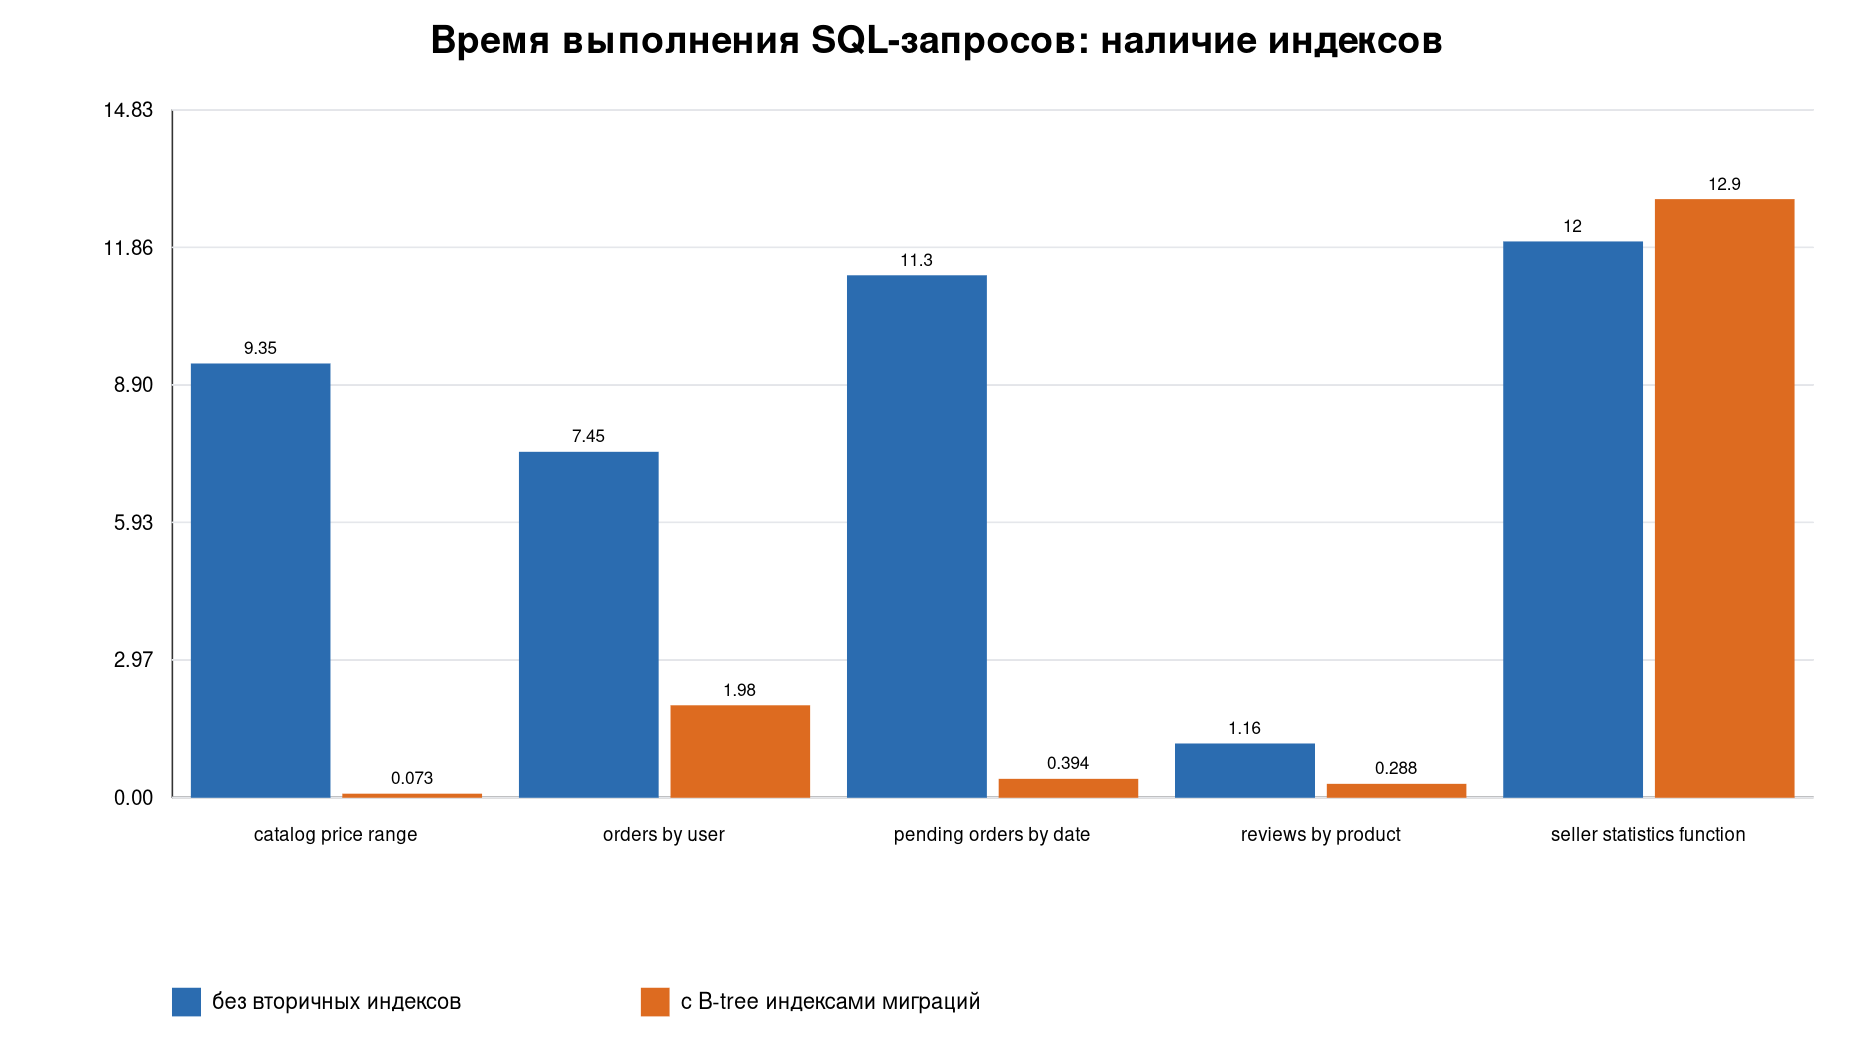
\includegraphics[width=0.9\textwidth]{research_presence.png}
    \caption{Время выполнения запросов при наличии и отсутствии индексов}
    \label{fig:research_presence}
\end{figure}

Для запросов с выборкой по индексируемому столбцу наличие индекса сокращает время выполнения на один--два порядка: планировщик переходит от последовательного сканирования (\texttt{Seq Scan}) к сканированию по индексу. Для хранимой функции статистики индексы из набора миграций не дают выигрыша, а в отдельных прогонах время незначительно возрастает: запрос соединяет три таблицы с агрегацией, и доступные индексы не покрывают его план. Это показывает, что индекс полезен не всегда и должен соответствовать конкретному запросу.

\subsection{Тип индекса: простой и составной}

Во втором подыспытании сравниваются простой индекс \texttt{(user\_id)} и составной \texttt{(user\_id, created\_at desc)} для запроса выборки заказов покупателя с сортировкой по дате. Результаты --- в таблице~\ref{tbl:research_type}.

При простом индексе план содержит узел сортировки (\texttt{Sort}): индекс отбирает строки покупателя, после чего они сортируются по дате. Составной индекс хранит строки уже в нужном порядке, поэтому узел сортировки из плана исчезает, а время выполнения снижается. Эффект проявляется при достаточном числе заказов у покупателя; на равномерном распределении он незаметен, поэтому заказы в наборе сконцентрированы на части покупателей.

\subsection{Тип индекса: B-tree и GIN для текстового поиска}

Третье подыспытание сравнивает два типа индекса для подстрочного поиска по имени товара (\texttt{name ILIKE '\%токен\%'}). Индекс B-tree для шаблона с ведущим символом подстановки неприменим, поэтому выполняется последовательное сканирование. Индекс GIN с классом операторов \texttt{gin\_trgm\_ops} (расширение \texttt{pg\_trgm}) индексирует триграммы и обслуживает такой поиск через \texttt{Bitmap Heap Scan}. Результаты --- в таблице~\ref{tbl:research_type}.

При низкой селективности запроса GIN-индекс сокращает время выполнения более чем на порядок относительно последовательного сканирования. Рисунок~\ref{fig:research_scaling} показывает, что разрыв растёт с увеличением числа товаров: время последовательного сканирования растёт линейно по размеру таблицы, а время поиска по GIN-индексу остаётся практически постоянным.

\begin{figure}[H]
    \centering
    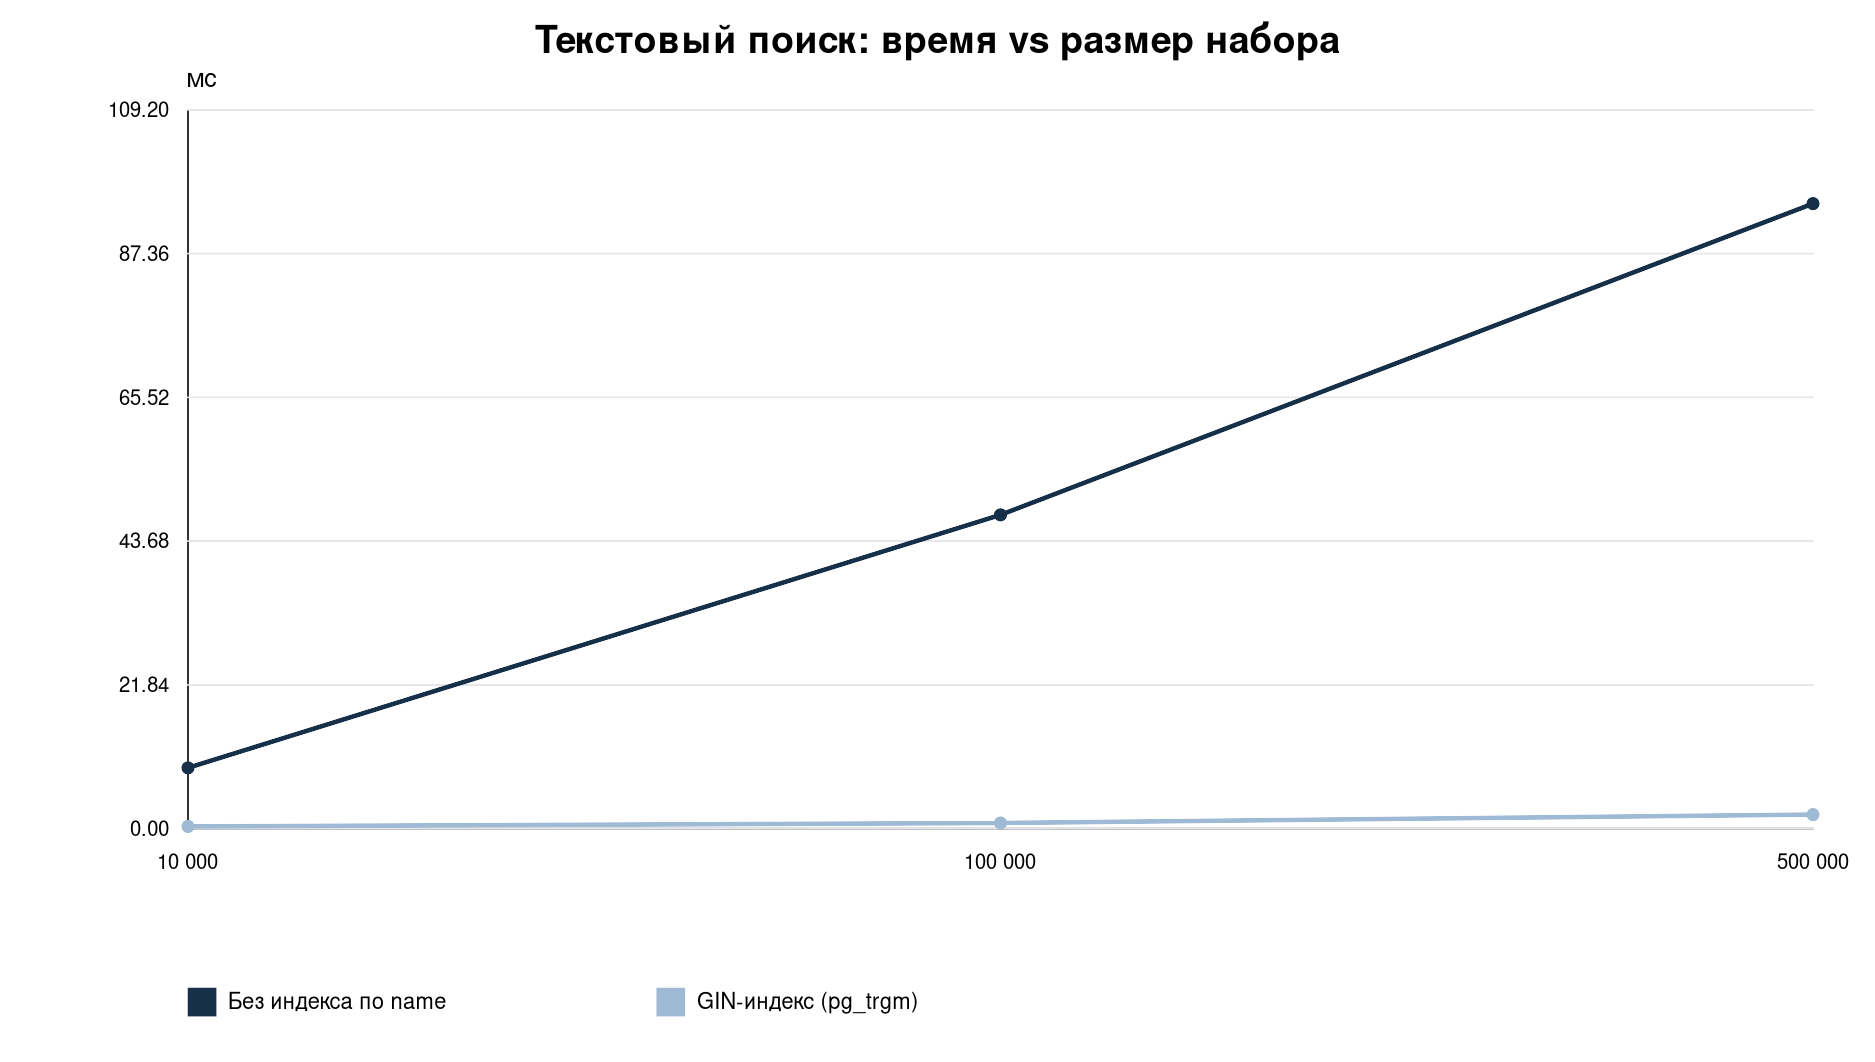
\includegraphics[width=0.9\textwidth]{research_scaling.png}
    \caption{Время текстового поиска в зависимости от размера набора: Seq Scan и GIN}
    \label{fig:research_scaling}
\end{figure}

\section{Исследование 2: влияние Redis-кэширования}

Во втором исследовании оценивается влияние внешнего кэша Redis на время отклика приложения. Нагрузка подаётся на четыре маршрута чтения: карточка товара, каталог, отзывы товара и список категорий. Сравниваются два сценария: Redis отключён и Redis включён с прогретым кэшем. Результаты приведены в таблице~\ref{tbl:research_http} и на рисунке~\ref{fig:research_http}; доля попаданий в кэш и относительное число обращений к PostgreSQL --- в таблице~\ref{tbl:research_cache_meta}.

\begin{figure}[H]
    \centering
    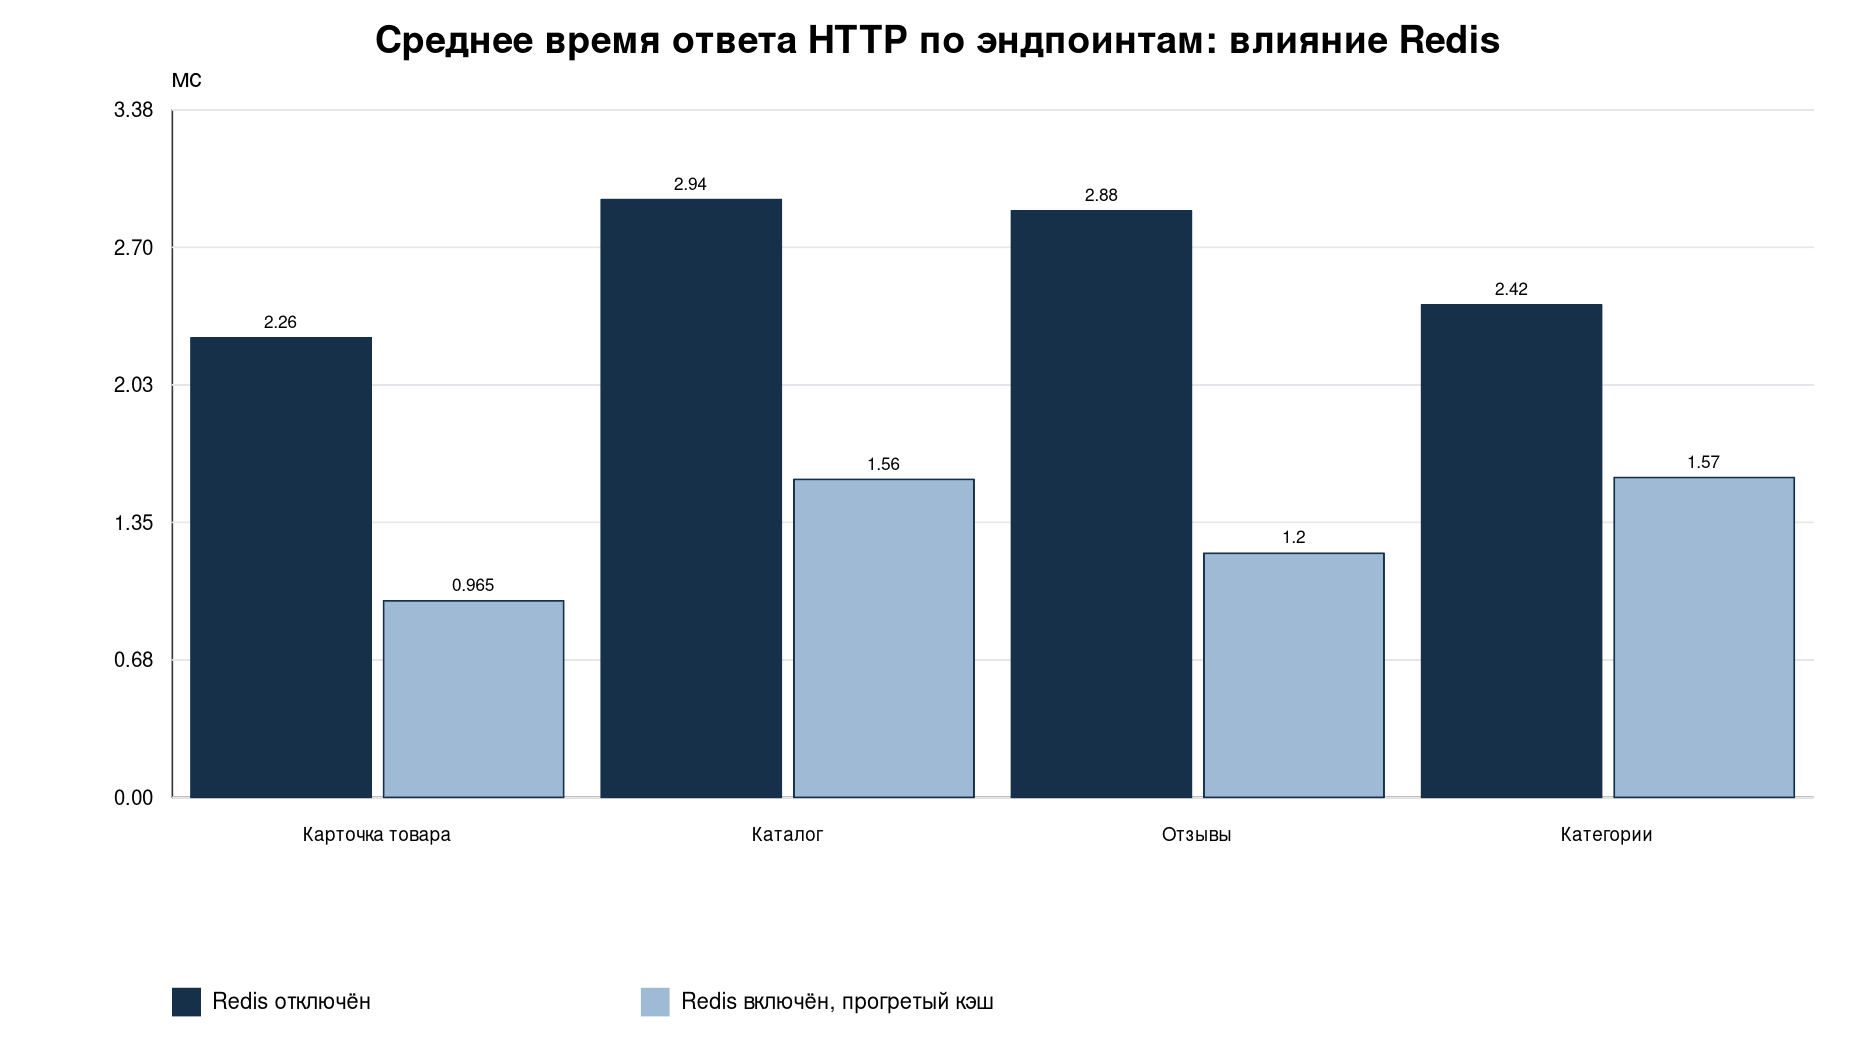
\includegraphics[width=0.9\textwidth]{research_http.png}
    \caption{Среднее время ответа по эндпоинтам: Redis отключён и включён}
    \label{fig:research_http}
\end{figure}

Включение кэша снижает среднее время ответа и, в большей степени, хвостовые перцентили \texttt{P95} и \texttt{P99}: повторные чтения обслуживаются из памяти, без обращения к PostgreSQL. При прогретом кэше доля попаданий близка к единице, а число строк, читаемых из PostgreSQL, снижается практически до нуля. Величина выигрыша зависит от маршрута (см. таблицу~\ref{tbl:research_http}): для часто запрашиваемой карточки товара относительное снижение времени наибольшее, тогда как для и без того дешёвого списка категорий эффект мал.

% Generated by scripts/research/render_results.py
\begin{table}[H]
\centering
\caption{Среднее время выполнения запросов при различном наборе индексов}
\label{tbl:research_presence}
\begin{tabular}{|p{0.32\textwidth}|p{0.40\textwidth}|r|}
\hline
Запрос & Вариант & Время, мс \\ \hline
catalog\_price\_range & без вторичных индексов & 9.351 \\ \hline
catalog\_price\_range & с B-tree индексами миграций & 0.073 \\ \hline
orders\_by\_user & без вторичных индексов & 7.448 \\ \hline
orders\_by\_user & с B-tree индексами миграций & 1.977 \\ \hline
pending\_orders\_by\_date & без вторичных индексов & 11.252 \\ \hline
pending\_orders\_by\_date & с B-tree индексами миграций & 0.394 \\ \hline
reviews\_by\_product & без вторичных индексов & 1.156 \\ \hline
reviews\_by\_product & с B-tree индексами миграций & 0.288 \\ \hline
seller\_statistics\_function & без вторичных индексов & 11.983 \\ \hline
seller\_statistics\_function & с B-tree индексами миграций & 12.894 \\ \hline
\end{tabular}
\end{table}

\begin{table}[H]
\centering
\caption{Влияние типа индекса на время выполнения}
\label{tbl:research_type}
\begin{tabular}{|p{0.42\textwidth}|c|p{0.22\textwidth}|r|}
\hline
Случай & Узел Sort & Корневой узел & Время, мс \\ \hline
orders\_by\_user: простой индекс (user\_id) & yes & Limit & 2.100 \\ \hline
orders\_by\_user: составной индекс (user\_id, created\_at desc) & no & Limit & 0.528 \\ \hline
text\_search: только B-tree (для '\%x\%' неприменим -> Seq Scan) & no & Seq Scan & 21.962 \\ \hline
text\_search: GIN + pg\_trgm & no & Bitmap Heap Scan & 0.442 \\ \hline
\end{tabular}
\end{table}

\begin{table}[H]
\centering
\caption{Время текстового поиска в зависимости от размера набора}
\label{tbl:research_scaling}
\begin{tabular}{|r|p{0.26\textwidth}|r|p{0.22\textwidth}|}
\hline
Размер & Вариант & Время, мс & Узел \\ \hline
10000 & Seq Scan (без GIN) & 9.234 & Seq Scan \\ \hline
10000 & GIN + pg\_trgm & 0.343 & Bitmap Heap Scan \\ \hline
100000 & Seq Scan (без GIN) & 47.672 & Seq Scan \\ \hline
100000 & GIN + pg\_trgm & 0.843 & Bitmap Heap Scan \\ \hline
500000 & Seq Scan (без GIN) & 94.959 & Gather \\ \hline
500000 & GIN + pg\_trgm & 2.148 & Bitmap Heap Scan \\ \hline
\end{tabular}
\end{table}

\begin{table}[H]
\centering
\caption{Нагрузочное тестирование: время ответа по эндпоинтам (влияние Redis)}
\label{tbl:research_http}
\begin{tabular}{|p{0.20\textwidth}|p{0.28\textwidth}|r|r|r|}
\hline
Эндпоинт & Сценарий & RPS & Среднее, мс & P99, мс \\ \hline
Карточка товара & Redis отключён & 4999.96 & 2.256 & 18.156 \\ \hline
Каталог & Redis отключён & 3893.96 & 2.935 & 11.712 \\ \hline
Отзывы & Redis отключён & 3977.65 & 2.879 & 5.590 \\ \hline
Категории & Redis отключён & 4596.96 & 2.417 & 4.439 \\ \hline
Карточка товара & Redis включён, прогретый кэш & 11019.35 & 0.965 & 2.638 \\ \hline
Каталог & Redis включён, прогретый кэш & 7135.62 & 1.561 & 3.389 \\ \hline
Отзывы & Redis включён, прогретый кэш & 9186.10 & 1.198 & 2.559 \\ \hline
Категории & Redis включён, прогретый кэш & 6872.77 & 1.570 & 3.200 \\ \hline
\end{tabular}
\end{table}

\begin{table}[H]
\centering
\caption{Доля попаданий в кэш и обращения к PostgreSQL}
\label{tbl:research_cache_meta}
\begin{tabular}{|p{0.34\textwidth}|r|r|r|}
\hline
Сценарий & Попаданий & Промахов & Доля попаданий \\ \hline
Redis отключён & 0 & 0 & 0.000 \\ \hline
Redis включён, прогретый кэш & 1500 & 0 & 1.000 \\ \hline
\end{tabular}
\end{table}


\section*{Вывод}
\addcontentsline{toc}{section}{Вывод}

Проведённое исследование показало, что индекс ускоряет выборку только при соответствии его структуры запросу: наличие индекса по фильтруемому столбцу сокращает время на один--два порядка, составной индекс дополнительно устраняет сортировку, а для подстрочного поиска требуется индекс типа GIN, тогда как B-tree неприменим. Внешний кэш Redis снижает время отклика приложения и особенно хвостовые задержки за счёт сокращения обращений к PostgreSQL, причём сильнее всего для дорогих запросов. PostgreSQL остаётся источником истины, а индексы и кэш выступают средствами оптимизации производительности в рамках одной и той же схемы данных.


% % !TEX root = ../report.tex

\ssr{ЗАКЛЮЧЕНИЕ}

В ходе выполнения курсового проекта была разработана база данных онлайн-маркетплейса и приложение доступа к ней.

В аналитической части рассмотрена предметная область, выполнено сравнение существующих решений, сформулированы требования и ограничения проектируемой системы. Выделены роли пользователей, сценарии взаимодействия, сущности и связи между ними. Для хранения данных выбрана реляционная модель.

В конструкторской части спроектированы таблицы базы данных, ограничения целостности, индексы, ролевая модель доступа, триггеры и хранимая функция. Выполнена проверка соответствия схемы третьей нормальной форме.

В технологической части описана реализация на PostgreSQL, Go и Redis. Реализованы миграции схемы, роли СУБД, триггеры, хранимая функция, REST API, серверный Web-интерфейс и кэширование часто читаемых данных по схеме Cache-Aside.

В исследовательской части выполнены измерения времени выполнения SQL-запросов при разных наборах индексов и времени HTTP-ответа при отключённом и прогретом Redis-кэше. Исследование показало, что индекс ускоряет запрос только при соответствии структуре условия и сортировки, а Redis-кэш снижает время ответа за счёт сокращения обращений к PostgreSQL.

Поставленная цель достигнута. Разработана база данных маркетплейса и приложение доступа к ней. Исследованы выбранные способы ускорения чтения данных.

\clearpage


\def\bibname{\begin{center}\Large СПИСОК ИСПОЛЬЗОВАННЫХ ИСТОЧНИКОВ\end{center}}

% !TEX root = ../report.tex

\begin{thebibliography}{99}
\sloppy

\bibitem{marketplace_def} Маркетплейс~// Википедия~--- свободная энциклопедия. URL: \url{https://ru.wikipedia.org/wiki/Marketplace} (дата обращения: 25.03.2026).

\bibitem{akit2025} АКИТ: объём интернет-торговли в России в 2025 году вырос на 28\%~// Rambler. URL: \url{https://finance.rambler.ru/economics/56067709-akit-obem-internet-torgovli-v-rossii-v-2025-godu-vyros-na-28/} (дата обращения: 25.03.2026).

\bibitem{ozon} Ozon Seller API Documentation. URL: \url{https://docs.ozon.ru/api/seller/} (дата обращения: 25.03.2026).

\bibitem{wildberries} Wildberries API для продавцов. URL: \url{https://dev.wildberries.ru} (дата обращения: 25.03.2026).

\bibitem{aliexpress} AliExpress Open Platform. URL: \url{https://openservice.aliexpress.com/doc/api.htm} (дата обращения: 25.03.2026).

\bibitem{ozon_vs_wb} Ozon vs Wildberries: сравнение маркетплейсов~// InSales. URL: \url{https://www.insales.ru/blogs/university/ozon-vs-wildberries} (дата обращения: 25.03.2026).

\bibitem{db_models} Дейт~К.\,Дж. Введение в системы баз данных~/ К.\,Дж.~Дейт.~--- 8-е изд.~--- М.\,: Вильямс, 2020.~--- 1328~с.

\bibitem{relation_model} Кодд~Э.\,Ф. Реляционная модель данных для больших совместно используемых банков данных~/ Э.\,Ф.~Кодд~// Communications of the ACM.~--- 1970.~--- Т.\,13, \textnumero\,6.~--- С.\,377--387.

\bibitem{postgresql_doc} PostgreSQL 16 Documentation. URL: \url{https://www.postgresql.org/docs/16/} (дата обращения: 25.03.2026).

\bibitem{redis_doc} Redis Documentation. URL: \url{https://redis.io/docs/} (дата обращения: 25.03.2026).

\end{thebibliography}


\end{document}
